%%%%%%%%%%%%%%%%%%%%%%%%%%%%%%%%%%%%%%%%%
% The Legrand Orange Book
% LaTeX Template
% Version 2.4 (26/09/2018)
%
% This template was downloaded from:
% http://www.LaTeXTemplates.com
%
% Original author:
% Mathias Legrand (legrand.mathias@gmail.com) with modifications by:
% Vel (vel@latextemplates.com)
%
% License:
% CC BY-NC-SA 3.0 (http://creativecommons.org/licenses/by-nc-sa/3.0/)
%
% Compiling this template:
% This template uses biber for its bibliography and makeindex for its index.
% When you first open the template, compile it from the command line with the 
% commands below to make sure your LaTeX distribution is configured correctly:
%
% 1) pdflatex main
% 2) makeindex main.idx -s StyleInd.ist
% 3) biber main
% 4) pdflatex main x 2
%
% After this, when you wish to update the bibliography/index use the appropriate
% command above and make sure to compile with pdflatex several times 
% afterwards to propagate your changes to the document.
%
% This template also uses a number of packages which may need to be
% updated to the newest versions for the template to compile. It is strongly
% recommended you update your LaTeX distribution if you have any
% compilation errors.
%
% Important note:
% Chapter heading images should have a 2:1 width:height ratio,
% e.g. 920px width and 460px height.
%
%%%%%%%%%%%%%%%%%%%%%%%%%%%%%%%%%%%%%%%%%

%----------------------------------------------------------------------------------------
%	PACKAGES AND OTHER DOCUMENT CONFIGURATIONS
%----------------------------------------------------------------------------------------

\documentclass[11pt,fleqn]{book} % Default font size and left-justified equations

%%%%%%%%%%%%%%%%%%%%%%%%%%%%%%%%%%%%%%%%%
% The Legrand Orange Book
% Structural Definitions File
% Version 2.1 (26/09/2018)
%
% Original author:
% Mathias Legrand (legrand.mathias@gmail.com) with modifications by:
% Vel (vel@latextemplates.com)
% 
% This file was downloaded from:
% http://www.LaTeXTemplates.com
%
% License:
% CC BY-NC-SA 3.0 (http://creativecommons.org/licenses/by-nc-sa/3.0/)
%
%%%%%%%%%%%%%%%%%%%%%%%%%%%%%%%%%%%%%%%%%

%----------------------------------------------------------------------------------------
%	VARIOUS REQUIRED PACKAGES AND CONFIGURATIONS
%----------------------------------------------------------------------------------------

\usepackage{graphicx} % Required for including pictures
\graphicspath{{Pictures/}} % Specifies the directory where pictures are stored

\usepackage{lipsum} % Inserts dummy text

\usepackage{tikz} % Required for drawing custom shapes

\usepackage[english]{babel} % English language/hyphenation

\usepackage{enumitem} % Customize lists
\setlist{nolistsep} % Reduce spacing between bullet points and numbered lists

\usepackage{booktabs} % Required for nicer horizontal rules in tables

\usepackage{xcolor} % Required for specifying colors by name
%\definecolor{ocre}{RGB}{40,122,255} % Define the orange color used for highlighting throughout the book
%\definecolor{ocre}{RGB}{20,30,150}			% A more neutral blue
\definecolor{ocre}{HTML}{2879c7}		%ippbleu

%----------------------------------------------------------------------------------------
%	MARGINS
%----------------------------------------------------------------------------------------

\usepackage{geometry} % Required for adjusting page dimensions and margins

\geometry{
	paper=a4paper, % Paper size, change to letterpaper for US letter size
	top=3cm, % Top margin
	bottom=3cm, % Bottom margin
	left=3cm, % Left margin
	right=3cm, % Right margin
	headheight=14pt, % Header height
	footskip=1.4cm, % Space from the bottom margin to the baseline of the footer
	headsep=10pt, % Space from the top margin to the baseline of the header
	%showframe, % Uncomment to show how the type block is set on the page
}

%----------------------------------------------------------------------------------------
%	FONTS
%----------------------------------------------------------------------------------------

% \usepackage{avant} % Use the Avantgarde font for headings
\usepackage{times} % Use the Times font for headings
\usepackage{mathptmx} % Use the Adobe Times Roman as the default text font together with math symbols from the Sym­bol, Chancery and Com­puter Modern fonts

\usepackage{microtype} % Slightly tweak font spacing for aesthetics
\usepackage[utf8]{inputenc} % Required for including letters with accents
\usepackage[T1]{fontenc} % Use 8-bit encoding that has 256 glyphs

%----------------------------------------------------------------------------------------
%	BIBLIOGRAPHY AND INDEX
%----------------------------------------------------------------------------------------

\usepackage[style=numeric,citestyle=numeric,sorting=nyt,sortcites=true,autopunct=true,babel=hyphen,hyperref=true,abbreviate=false,backref=true,backend=biber]{biblatex}
\addbibresource{bibliography.bib} % BibTeX bibliography file
\defbibheading{bibempty}{}

\usepackage{calc} % For simpler calculation - used for spacing the index letter headings correctly
\usepackage{makeidx} % Required to make an index
\makeindex % Tells LaTeX to create the files required for indexing

%----------------------------------------------------------------------------------------
%	MAIN TABLE OF CONTENTS
%----------------------------------------------------------------------------------------

\usepackage{titletoc} % Required for manipulating the table of contents

\contentsmargin{0cm} % Removes the default margin

% Part text styling (this is mostly taken care of in the PART HEADINGS section of this file)
\titlecontents{part}
	[0cm] % Left indentation
	{\addvspace{20pt}\bfseries} % Spacing and font options for parts
	{}
	{}
	{}

% Chapter text styling
\titlecontents{chapter}
	[1.25cm] % Left indentation
	{\addvspace{12pt}\large\sffamily\bfseries} % Spacing and font options for chapters
	{\color{ocre!60}\contentslabel[\Large\thecontentslabel]{1.25cm}\color{ocre}} % Formatting of numbered sections of this type
	{\color{ocre}} % Formatting of numberless sections of this type
	{\color{ocre!60}\normalsize\;\titlerule*[.5pc]{.}\;\thecontentspage} % Formatting of the filler to the right of the heading and the page number

% Section text styling
\titlecontents{section}
	[1.25cm] % Left indentation
	{\addvspace{3pt}\sffamily\bfseries} % Spacing and font options for sections
	{\contentslabel[\thecontentslabel]{1.25cm}} % Formatting of numbered sections of this type
	{} % Formatting of numberless sections of this type
	{\hfill\color{black}\thecontentspage} % Formatting of the filler to the right of the heading and the page number

% Subsection text styling
\titlecontents{subsection}
	[1.25cm] % Left indentation
	{\addvspace{1pt}\sffamily\small} % Spacing and font options for subsections
	{\contentslabel[\thecontentslabel]{1.25cm}} % Formatting of numbered sections of this type
	{} % Formatting of numberless sections of this type
	{\ \titlerule*[.5pc]{.}\;\thecontentspage} % Formatting of the filler to the right of the heading and the page number

% Figure text styling
\titlecontents{figure}
	[1.25cm] % Left indentation
	{\addvspace{1pt}\sffamily\small} % Spacing and font options for figures
	{\thecontentslabel\hspace*{1em}} % Formatting of numbered sections of this type
	{} % Formatting of numberless sections of this type
	{\ \titlerule*[.5pc]{.}\;\thecontentspage} % Formatting of the filler to the right of the heading and the page number

% Table text styling
\titlecontents{table}
	[1.25cm] % Left indentation
	{\addvspace{1pt}\sffamily\small} % Spacing and font options for tables
	{\thecontentslabel\hspace*{1em}} % Formatting of numbered sections of this type
	{} % Formatting of numberless sections of this type
	{\ \titlerule*[.5pc]{.}\;\thecontentspage} % Formatting of the filler to the right of the heading and the page number

%----------------------------------------------------------------------------------------
%	MINI TABLE OF CONTENTS IN PART HEADS
%----------------------------------------------------------------------------------------

% Chapter text styling
\titlecontents{lchapter}
	[0em] % Left indentation
	{\addvspace{15pt}\large\sffamily\bfseries} % Spacing and font options for chapters
	{\color{ocre}\contentslabel[\Large\thecontentslabel]{1.25cm}\color{ocre}} % Chapter number
	{}  
	{\color{ocre}\normalsize\sffamily\bfseries\;\titlerule*[.5pc]{.}\;\thecontentspage} % Page number

% Section text styling
\titlecontents{lsection}
	[0em] % Left indentation
	{\sffamily\small} % Spacing and font options for sections
	{\contentslabel[\thecontentslabel]{1.25cm}} % Section number
	{}
	{}

% Subsection text styling (note these aren't shown by default, display them by searchings this file for tocdepth and reading the commented text)
\titlecontents{lsubsection}
	[.5em] % Left indentation
	{\sffamily\footnotesize} % Spacing and font options for subsections
	{\contentslabel[\thecontentslabel]{1.25cm}}
	{}
	{}

%----------------------------------------------------------------------------------------
%	HEADERS AND FOOTERS
%----------------------------------------------------------------------------------------

\usepackage{fancyhdr} % Required for header and footer configuration

\pagestyle{fancy} % Enable the custom headers and footers

\renewcommand{\chaptermark}[1]{\markboth{\sffamily\normalsize\bfseries\chaptername\ \thechapter.\ #1}{}} % Styling for the current chapter in the header
\renewcommand{\sectionmark}[1]{\markright{\sffamily\normalsize\thesection\hspace{5pt}#1}{}} % Styling for the current section in the header

\fancyhf{} % Clear default headers and footers
\fancyhead[LE,RO]{\sffamily\normalsize\thepage} % Styling for the page number in the header
\fancyhead[LO]{\rightmark} % Print the nearest section name on the left side of odd pages
\fancyhead[RE]{\leftmark} % Print the current chapter name on the right side of even pages
%\fancyfoot[C]{\thepage} % Uncomment to include a footer

\renewcommand{\headrulewidth}{0.5pt} % Thickness of the rule under the header

\fancypagestyle{plain}{% Style for when a plain pagestyle is specified
	\fancyhead{}\renewcommand{\headrulewidth}{0pt}%
}

% Removes the header from odd empty pages at the end of chapters
\makeatletter
\renewcommand{\cleardoublepage}{
\clearpage\ifodd\c@page\else
\hbox{}
\vspace*{\fill}
\thispagestyle{empty}
%\newpage
\fi}

%----------------------------------------------------------------------------------------
%	THEOREM STYLES
%----------------------------------------------------------------------------------------

\usepackage{amsmath,amsfonts,amssymb,amsthm} % For math equations, theorems, symbols, etc

\newcommand{\intoo}[2]{\mathopen{]}#1\,;#2\mathclose{[}}
\newcommand{\ud}{\mathop{\mathrm{{}d}}\mathopen{}}
\newcommand{\intff}[2]{\mathopen{[}#1\,;#2\mathclose{]}}
\renewcommand{\qedsymbol}{$\blacksquare$}
\newtheorem{notation}{Notation}[chapter]

% Boxed/framed environments
\newtheoremstyle{ocrenumbox}% Theorem style name
{0pt}% Space above
{0pt}% Space below
{\normalfont}% Body font
{}% Indent amount
{\small\bf\sffamily\color{ocre}}% Theorem head font
{\;}% Punctuation after theorem head
{0.25em}% Space after theorem head
{\small\sffamily\color{ocre}\thmname{#1}\nobreakspace\thmnumber{\@ifnotempty{#1}{}\@upn{#2}}% Theorem text (e.g. Theorem 2.1)
\thmnote{\nobreakspace\the\thm@notefont\sffamily\bfseries\color{black}---\nobreakspace#3.}} % Optional theorem note

\newtheoremstyle{blacknumex}% Theorem style name
{5pt}% Space above
{5pt}% Space below
{\normalfont}% Body font
{} % Indent amount
{\small\bf\sffamily}% Theorem head font
{\;}% Punctuation after theorem head
{0.25em}% Space after theorem head
{\small\sffamily{\tiny\ensuremath{\blacksquare}}\nobreakspace\thmname{#1}\nobreakspace\thmnumber{\@ifnotempty{#1}{}\@upn{#2}}% Theorem text (e.g. Theorem 2.1)
\thmnote{\nobreakspace\the\thm@notefont\sffamily\bfseries---\nobreakspace#3.}}% Optional theorem note

\newtheoremstyle{blacknumbox} % Theorem style name
{0pt}% Space above
{0pt}% Space below
{\normalfont}% Body font
{}% Indent amount
{\small\bf\sffamily}% Theorem head font
{\;}% Punctuation after theorem head
{0.25em}% Space after theorem head
{\small\sffamily\thmname{#1}\nobreakspace\thmnumber{\@ifnotempty{#1}{}\@upn{#2}}% Theorem text (e.g. Theorem 2.1)
\thmnote{\nobreakspace\the\thm@notefont\sffamily\bfseries---\nobreakspace#3.}}% Optional theorem note

% Non-boxed/non-framed environments
\newtheoremstyle{ocrenum}% Theorem style name
{5pt}% Space above
{5pt}% Space below
{\normalfont}% Body font
{}% Indent amount
{\small\bf\sffamily\color{ocre}}% Theorem head font
{\;}% Punctuation after theorem head
{0.25em}% Space after theorem head
{\small\sffamily\color{ocre}\thmname{#1}\nobreakspace\thmnumber{\@ifnotempty{#1}{}\@upn{#2}}% Theorem text (e.g. Theorem 2.1)
\thmnote{\nobreakspace\the\thm@notefont\sffamily\bfseries\color{black}---\nobreakspace#3.}} % Optional theorem note
\makeatother

% Defines the theorem text style for each type of theorem to one of the three styles above
\newcounter{dummy} 
\numberwithin{dummy}{section}
\theoremstyle{ocrenumbox}
\newtheorem{theoremeT}[dummy]{Theorem}
\newtheorem{problem}{Problem}[chapter]
\newtheorem{exerciseT}{Exercise}[chapter]
\theoremstyle{blacknumex}
\newtheorem{exampleT}{Example}[chapter]
\theoremstyle{blacknumbox}
\newtheorem{vocabulary}{Vocabulary}[chapter]
\newtheorem{definitionT}{Definition}[section]
\newtheorem{corollaryT}[dummy]{Corollary}
\theoremstyle{ocrenum}
\newtheorem{proposition}[dummy]{Proposition}

%----------------------------------------------------------------------------------------
%	DEFINITION OF COLORED BOXES
%----------------------------------------------------------------------------------------

\RequirePackage[framemethod=default]{mdframed} % Required for creating the theorem, definition, exercise and corollary boxes

% Theorem box
\newmdenv[skipabove=7pt,
skipbelow=7pt,
backgroundcolor=black!5,
linecolor=ocre,
innerleftmargin=5pt,
innerrightmargin=5pt,
innertopmargin=5pt,
leftmargin=0cm,
rightmargin=0cm,
innerbottommargin=5pt]{tBox}

% Exercise box	  
\newmdenv[skipabove=7pt,
skipbelow=7pt,
rightline=false,
leftline=true,
topline=false,
bottomline=false,
backgroundcolor=ocre!10,
linecolor=ocre,
innerleftmargin=5pt,
innerrightmargin=5pt,
innertopmargin=5pt,
innerbottommargin=5pt,
leftmargin=0cm,
rightmargin=0cm,
linewidth=4pt]{eBox}	

% Definition box
\newmdenv[skipabove=7pt,
skipbelow=7pt,
rightline=false,
leftline=true,
topline=false,
bottomline=false,
linecolor=ocre,
innerleftmargin=5pt,
innerrightmargin=5pt,
innertopmargin=0pt,
leftmargin=0cm,
rightmargin=0cm,
linewidth=4pt,
innerbottommargin=0pt]{dBox}	

% Corollary box
\newmdenv[skipabove=7pt,
skipbelow=7pt,
rightline=false,
leftline=true,
topline=false,
bottomline=false,
linecolor=gray,
backgroundcolor=black!5,
innerleftmargin=5pt,
innerrightmargin=5pt,
innertopmargin=5pt,
leftmargin=0cm,
rightmargin=0cm,
linewidth=4pt,
innerbottommargin=5pt]{cBox}

% Equation box
\newmdenv[skipabove=2pt,
skipbelow=7pt,
backgroundcolor=black!5,
linecolor=ocre,
innerleftmargin=5pt,
innerrightmargin=5pt,
innertopmargin=-8pt,
leftmargin=0cm,
rightmargin=0cm,
innerbottommargin=5pt]{eqBox}

% Creates an environment for each type of theorem and assigns it a theorem text style from the "Theorem Styles" section above and a colored box from above
\newenvironment{theorem}{\begin{tBox}\begin{theoremeT}}{\end{theoremeT}\end{tBox}}
\newenvironment{exercise}{\begin{eBox}\begin{exerciseT}}{\hfill{\color{ocre}\tiny\ensuremath{\blacksquare}}\end{exerciseT}\end{eBox}}				  
\newenvironment{definition}{\begin{dBox}\begin{definitionT}}{\end{definitionT}\end{dBox}}	
\newenvironment{example}{\begin{exampleT}}{\hfill{\tiny\ensuremath{\blacksquare}}\end{exampleT}}		
\newenvironment{corollary}{\begin{cBox}\begin{corollaryT}}{\end{corollaryT}\end{cBox}}	

%----------------------------------------------------------------------------------------
%	REMARK ENVIRONMENT
%----------------------------------------------------------------------------------------

\newenvironment{remark}{\par\vspace{10pt}\small % Vertical white space above the remark and smaller font size
\begin{list}{}{
\leftmargin=35pt % Indentation on the left
\rightmargin=25pt}\item\ignorespaces % Indentation on the right
\makebox[-2.5pt]{\begin{tikzpicture}[overlay]
\node[draw=ocre!60,line width=1pt,circle,fill=ocre!25,font=\sffamily\bfseries,inner sep=2pt,outer sep=0pt] at (-15pt,0pt){\textcolor{ocre}{R}};\end{tikzpicture}} % Orange R in a circle
\advance\baselineskip -1pt}{\end{list}\vskip5pt} % Tighter line spacing and white space after remark

%----------------------------------------------------------------------------------------
%	JUPYTER NOTEBOOK ENVIRONMENT
%----------------------------------------------------------------------------------------

\newenvironment{jupyternote}{\par\vspace{10pt}\small % Vertical white space above the remark and smaller font size
\begin{list}{}{
\leftmargin=35pt % Indentation on the left
\rightmargin=25pt}\item\ignorespaces % Indentation on the right
\makebox[-2.5pt]{\begin{tikzpicture}[overlay]
\node[draw=ocre!60,line width=1pt,circle,fill=none,font=\sffamily\bfseries,inner sep=0pt,outer sep=0pt] at (-15pt,0pt){
\includegraphics[width=.04\textwidth]{Pictures/jupyter_logo}};\end{tikzpicture}\quad} % Orange R in a circle
\advance\baselineskip -1pt}{\end{list}\vskip5pt} % Tighter line spacing and white space after remark

%----------------------------------------------------------------------------------------
%	SU2 ENVIRONMENT
%----------------------------------------------------------------------------------------

\newenvironment{su2note}{\par\vspace{10pt}\small % Vertical white space above the remark and smaller font size
\begin{list}{}{
\leftmargin=35pt % Indentation on the left
\rightmargin=25pt}\item\ignorespaces % Indentation on the right
\makebox[-2.5pt]{\begin{tikzpicture}[overlay]
\node[draw=ocre!60,line width=1pt,circle,fill=none,font=\sffamily\bfseries,inner sep=0pt,outer sep=0pt] at (-15pt,0pt){\includegraphics[height=.03\textwidth]{Pictures/logoSU2}};\end{tikzpicture}\quad} % Orange R in a circle
\advance\baselineskip -1pt}{\end{list}\vskip5pt} % Tighter line spacing and white space after remark

%----------------------------------------------------------------------------------------
%	Gmsh ENVIRONMENT
%----------------------------------------------------------------------------------------

\newenvironment{gmshnote}{\par\vspace{10pt}\small % Vertical white space above the remark and smaller font size
\begin{list}{}{
\leftmargin=35pt % Indentation on the left
\rightmargin=25pt}\item\ignorespaces % Indentation on the right
\makebox[-2.5pt]{\begin{tikzpicture}[overlay]
\node[draw=ocre!60,line width=1pt,circle,fill=none,font=\sffamily\bfseries,inner sep=0pt,outer sep=0pt] at (-15pt,0pt){
\includegraphics[height=.04\textwidth]{Pictures/gmshlogo}};\end{tikzpicture}\quad} % Orange R in a circle
\advance\baselineskip -1pt}{\end{list}\vskip5pt} % Tighter line spacing and white space after remark

%----------------------------------------------------------------------------------------
%	Python ENVIRONMENT
%----------------------------------------------------------------------------------------

\newenvironment{pythonnote}{\par\vspace{10pt}\small % Vertical white space above the remark and smaller font size
\begin{list}{}{
\leftmargin=35pt % Indentation on the left
\rightmargin=25pt}\item\ignorespaces % Indentation on the right
\makebox[-2.5pt]{\begin{tikzpicture}[overlay]
\node[draw=ocre!60,line width=1pt,circle,fill=none,font=\sffamily\bfseries,inner sep=0pt,outer sep=0pt] at (-15pt,0pt){
\includegraphics[height=.04\textwidth]{Pictures/pythonlogo}};\end{tikzpicture}\quad} % Orange R in a circle
\advance\baselineskip -1pt}{\end{list}\vskip5pt} % Tighter line spacing and white space after remark

%----------------------------------------------------------------------------------------
%	Paraview ENVIRONMENT
%----------------------------------------------------------------------------------------

\newenvironment{paraviewnote}{\par\vspace{10pt}\small % Vertical white space above the remark and smaller font size
\begin{list}{}{
\leftmargin=35pt % Indentation on the left
\rightmargin=25pt}\item\ignorespaces % Indentation on the right
\makebox[-2.5pt]{\begin{tikzpicture}[overlay]
\node[draw=ocre!60,line width=1pt,circle,fill=none,font=\sffamily\bfseries,inner sep=0pt,outer sep=0pt] at (-15pt,0pt){
\includegraphics[height=.04\textwidth]{Pictures/paraviewlogo}};\end{tikzpicture}\quad} % Orange R in a circle
\advance\baselineskip -1pt}{\end{list}\vskip5pt} % Tighter line spacing and white space after remark

%----------------------------------------------------------------------------------------
%	SECTION NUMBERING IN THE MARGIN
%----------------------------------------------------------------------------------------

\makeatletter
\renewcommand{\@seccntformat}[1]{\llap{\textcolor{ocre}{\csname the#1\endcsname}\hspace{1em}}}                    
\renewcommand{\section}{\@startsection{section}{1}{\z@}
{-4ex \@plus -1ex \@minus -.4ex}
{1ex \@plus.2ex }
{\normalfont\large\sffamily\bfseries}}
\renewcommand{\subsection}{\@startsection {subsection}{2}{\z@}
{-3ex \@plus -0.1ex \@minus -.4ex}
{0.5ex \@plus.2ex }
{\normalfont\sffamily\bfseries}}
\renewcommand{\subsubsection}{\@startsection {subsubsection}{3}{\z@}
{-2ex \@plus -0.1ex \@minus -.2ex}
{.2ex \@plus.2ex }
{\normalfont\small\sffamily\bfseries}}                        
\renewcommand\paragraph{\@startsection{paragraph}{4}{\z@}
{-2ex \@plus-.2ex \@minus .2ex}
{.1ex}
{\normalfont\small\sffamily\bfseries}}

%----------------------------------------------------------------------------------------
%	PART HEADINGS
%----------------------------------------------------------------------------------------

% Numbered part in the table of contents
\newcommand{\@mypartnumtocformat}[2]{%
	\setlength\fboxsep{0pt}%
	\noindent\colorbox{ocre!20}{\strut\parbox[c][.7cm]{\ecart}{\color{ocre!70}\Large\sffamily\bfseries\centering#1}}\hskip\esp\colorbox{ocre!40}{\strut\parbox[c][.7cm]{\linewidth-\ecart-\esp}{\Large\sffamily\centering#2}}%
}

% Unnumbered part in the table of contents
\newcommand{\@myparttocformat}[1]{%
	\setlength\fboxsep{0pt}%
	\noindent\colorbox{ocre!40}{\strut\parbox[c][.7cm]{\linewidth}{\Large\sffamily\centering#1}}%
}

\newlength\esp
\setlength\esp{4pt}
\newlength\ecart
\setlength\ecart{1.2cm-\esp}
\newcommand{\thepartimage}{}%
\newcommand{\partimage}[1]{\renewcommand{\thepartimage}{#1}}%
\def\@part[#1]#2{%
\ifnum \c@secnumdepth >-2\relax%
\refstepcounter{part}%
\addcontentsline{toc}{part}{\texorpdfstring{\protect\@mypartnumtocformat{\thepart}{#1}}{\partname~\thepart\ ---\ #1}}
\else%
\addcontentsline{toc}{part}{\texorpdfstring{\protect\@myparttocformat{#1}}{#1}}%
\fi%
\startcontents%
\markboth{}{}%
{\thispagestyle{empty}%
\begin{tikzpicture}[remember picture,overlay]%
\node at (current page.north west){\begin{tikzpicture}[remember picture,overlay]%	
\fill[ocre!20](0cm,0cm) rectangle (\paperwidth,-\paperheight);
\node[anchor=north] at (4cm,-3.25cm){\color{ocre!40}\fontsize{220}{100}\sffamily\bfseries\thepart}; 
\node[anchor=south east] at (\paperwidth-1cm,-\paperheight+1cm){\parbox[t][][t]{8.5cm}{
\printcontents{l}{0}{\setcounter{tocdepth}{1}}% The depth to which the Part mini table of contents displays headings; 0 for chapters only, 1 for chapters and sections and 2 for chapters, sections and subsections
}};
\node[anchor=north east] at (\paperwidth-1.5cm,-3.25cm){\parbox[t][][t]{15cm}{\strut\raggedleft\color{white}\fontsize{30}{30}\sffamily\bfseries#2}};
\end{tikzpicture}};
\end{tikzpicture}}%
\@endpart}
\def\@spart#1{%
\startcontents%
\phantomsection
{\thispagestyle{empty}%
\begin{tikzpicture}[remember picture,overlay]%
\node at (current page.north west){\begin{tikzpicture}[remember picture,overlay]%	
\fill[ocre!20](0cm,0cm) rectangle (\paperwidth,-\paperheight);
\node[anchor=north east] at (\paperwidth-1.5cm,-3.25cm){\parbox[t][][t]{15cm}{\strut\raggedleft\color{white}\fontsize{30}{30}\sffamily\bfseries#1}};
\end{tikzpicture}};
\end{tikzpicture}}
\addcontentsline{toc}{part}{\texorpdfstring{%
\setlength\fboxsep{0pt}%
\noindent\protect\colorbox{ocre!40}{\strut\protect\parbox[c][.7cm]{\linewidth}{\Large\sffamily\protect\centering #1\quad\mbox{}}}}{#1}}%
\@endpart}
\def\@endpart{\vfil\newpage
\if@twoside
\if@openright
\null
\thispagestyle{empty}%
\newpage
\fi
\fi
\if@tempswa
\twocolumn
\fi}

%----------------------------------------------------------------------------------------
%	CHAPTER HEADINGS
%----------------------------------------------------------------------------------------

% A switch to conditionally include a picture, implemented by Christian Hupfer
\newif\ifusechapterimage
\usechapterimagetrue
\newcommand{\thechapterimage}{}%
\newcommand{\chapterimage}[1]{\ifusechapterimage\renewcommand{\thechapterimage}{#1}\fi}%
\newcommand{\autodot}{.}
\def\@makechapterhead#1{%
{\parindent \z@ \raggedright \normalfont
\ifnum \c@secnumdepth >\m@ne
\if@mainmatter
\begin{tikzpicture}[remember picture,overlay]
\node at (current page.north west)
{\begin{tikzpicture}[remember picture,overlay]
\node[anchor=north west,inner sep=0pt] at (0,0) {\ifusechapterimage\includegraphics[width=\paperwidth]{\thechapterimage}\fi};
\draw[anchor=west] (\Gm@lmargin,-9cm) node [line width=2pt,draw=ocre,fill=white,fill opacity=0.5,inner sep=15pt]{\strut\makebox[22cm]{}};
\draw[anchor=west] (\Gm@lmargin+.3cm,-9cm) node {\huge\sffamily\bfseries\color{black}\thechapter\autodot~#1\strut};
\end{tikzpicture}};
\end{tikzpicture}
\else
\begin{tikzpicture}[remember picture,overlay]
\node at (current page.north west)
{\begin{tikzpicture}[remember picture,overlay]
\node[anchor=north west,inner sep=0pt] at (0,0) {\ifusechapterimage\includegraphics[width=\paperwidth]{\thechapterimage}\fi};
\draw[anchor=west] (\Gm@lmargin,-9cm) node [line width=2pt,draw=ocre,fill=white,fill opacity=0.5,inner sep=15pt]{\strut\makebox[22cm]{}};
\draw[anchor=west] (\Gm@lmargin+.3cm,-9cm) node {\huge\sffamily\bfseries\color{black}#1\strut};
\end{tikzpicture}};
\end{tikzpicture}
\fi\fi\par\vspace*{270\p@}}}

%-------------------------------------------

\def\@makeschapterhead#1{%
\begin{tikzpicture}[remember picture,overlay]
\node at (current page.north west)
{\begin{tikzpicture}[remember picture,overlay]
\node[anchor=north west,inner sep=0pt] at (0,0) {\ifusechapterimage\includegraphics[width=\paperwidth]{\thechapterimage}\fi};
\draw[anchor=west] (\Gm@lmargin,-9cm) node [line width=2pt,draw=ocre,fill=white,fill opacity=0.5,inner sep=15pt]{\strut\makebox[22cm]{}};
\draw[anchor=west] (\Gm@lmargin+.3cm,-9cm) node {\huge\sffamily\bfseries\color{black}#1\strut};
\end{tikzpicture}};
\end{tikzpicture}
\par\vspace*{270\p@}}
\makeatother

%----------------------------------------------------------------------------------------
%	LINKS
%----------------------------------------------------------------------------------------

\usepackage{hyperref}
\hypersetup{hidelinks,backref=true,pagebackref=true,hyperindex=true,colorlinks=false,breaklinks=true,urlcolor=ocre,bookmarks=true,bookmarksopen=false}

\usepackage{bookmark}
\bookmarksetup{
open,
numbered,
addtohook={%
\ifnum\bookmarkget{level}=0 % chapter
\bookmarksetup{bold}%
\fi
\ifnum\bookmarkget{level}=-1 % part
\bookmarksetup{color=ocre,bold}%
\fi
}
}

\DeclareMathOperator{\di}{d\!}
\newcommand*\Eval[3]{\left.#1\right\rvert_{#2}^{#3}}
 % Insert the commands.tex file which contains the majority of the structure behind the template
\usepackage{subcaption}
\usepackage{float}
\hypersetup{pdftitle={BOOK TITLE},pdfauthor={Al-Khwarizmi}} % Uncomment and fill out to include PDF metadata for the author and title of the book

%----------------------------------------------------------------------------------------

%----------------------------------------------------------------------------------------
%	USEFUL TEXT VARIABLES
%----------------------------------------------------------------------------------------

\newcommand{\repourl}{https://gitlab.com/bvermeir/book-cfd}
\newcommand{\binderurl}{https://tinyurl.com/cfd-binder}

%----------------------------------------------------------------------------------------
%	USEFUL commands 
%----------------------------------------------------------------------------------------
\usepackage[ruled,vlined,linesnumbered]{algorithm2e}
\usepackage{bm}
\usepackage{tcolorbox} % box that includes text + math formula

\newtheorem{lemma}{Lemma}
\newcommand{\todo}[1]{\textcolor{red}{#1}}

\newcommand{\nn}{\bm{n}}
\newcommand{\ww}{\bm{w}}
\newcommand{\ee}{\bm{e}}
\newcommand{\ff}{\bm{f}}
\newcommand{\uu}{\bm{u}}
\newcommand{\vv}{\bm{v}}
\newcommand{\ii}{\bm{i}}
\newcommand{\jj}{\bm{j}}
\newcommand{\pp}{\bm{p}}
\newcommand{\kk}{\bm{k}}
\newcommand{\xx}{\bm{x}}
\newcommand{\UU}{\bm{U}}
\newcommand{\EE}{\bm{E}}
\newcommand{\FF}{\bm{F}}
\newcommand{\HH}{\bm{H}}
\newcommand{\GG}{\bm{G}}
\newcommand{\JJ}{\bm{J}}
\newcommand{\DD}{\bm{D}}
\newcommand{\BB}{\bm{B}}
\newcommand{\dotphi}{\dot{\phi}}
\newcommand{\PsiPsi}{\boldsymbol{\Psi}}
\newcommand{\etaeta}{\boldsymbol{\eta}}
\newcommand{\ttheta}{\bm{\theta}}
\newcommand{\mumu}{\boldsymbol{\mu}}
\newcommand{\xixi}{\boldsymbol{\xi}}
\newcommand{\intline}{\int_{\mathbb{R}}}
\newcommand{\fracp}[2]{\frac{\partial #1}{\partial #2}}
\newcommand{\dd}{\,{\rm d} }
\newcommand{\diff}{\mathrm{d}\,}
\newcommand{\Rotv}{\boldsymbol{\nabla} \times}
\newcommand{\Rots}{\nabla \times}
\newcommand{\Curl}{\nabla \times}
\newcommand{\Div}{\nabla \cdot}
\newcommand{\Grad}{\boldsymbol{\nabla}}
\newcommand{\Gradh}{\mathbb{G}}
\newcommand{\Curlvh}{\pmb{\mathbb{C}}}
\newcommand{\Curlh}{\mathbb{C}}
\newcommand{\Divh}{\mathbb{D}}
\newcommand{\Hgrad}{H^1(\Omega)}
\newcommand{\Hgradv}{\bm{H}^1(\Omega)}
\newcommand{\Hcurl}{\bm{H}(\mbox{curl}, \Omega)}
\newcommand{\Hdiv}{\bm{H}(\mbox{div}, \Omega)}
\newcommand{\Ltwo}{L^2(\Omega)}
\newcommand{\Ltwov}{\bm{L}^2(\Omega)}
\newcommand{\Hgradzero}{H^1_0(\Omega)}
\newcommand{\Hgradvzero}{\bm{H}^1_0(\Omega)}
\newcommand{\Hcurlzero}{\bm{H}_0(\mbox{curl}, \Omega)}
\newcommand{\Hdivzero}{\bm{H}_0(\mbox{div}, \Omega)}
\newcommand{\Ltwozero}{L^2_0(\Omega)}
\newcommand{\Ltwovzero}{\bm{L}^2_0(\Omega)}
\newcommand{\Vgrad}{V_h(\mbox{grad}, \Omega)}
\newcommand{\Vgradv}{\bm{V}_h(\mbox{grad}, \Omega)}
\newcommand{\Vcurl}{\bm{V}_h(\mbox{curl}, \Omega)}
\newcommand{\Vdiv}{\bm{V}_h(\mbox{div}, \Omega)}
\newcommand{\Vltwo}{V_h(L^2, \Omega)}
\newcommand{\Cinfinity}{\mathcal{C}^{\infty}(\Omega)}
\newcommand{\HgradLogical}{H^1(\hat{\Omega})}
\newcommand{\HcurlLogical}{{H}(\mbox{curl}, \hat{\Omega})}
\newcommand{\HdivLogical}{{H}(\mbox{div}, \hat{\Omega})}
\newcommand{\LtwoLogical}{L^2(\hat{\Omega})}
\newcommand{\VgradLogical}{V_h(\mbox{grad}, \hat{\Omega})}
\newcommand{\VcurlLogical}{{V}_h(\mbox{curl}, \hat{\Omega})}
\newcommand{\VdivLogical}{{V}_h(\mbox{div}, \hat{\Omega})}
\newcommand{\VltwoLogical}{V_h(L^2, \hat{\Omega})}
\newcommand{\igrad}{\imath^{0}}
\newcommand{\icurl}{\imath^{1}}
\newcommand{\idiv}{\imath^{2}}
\newcommand{\iltwo}{\imath^{3}}
\newcommand{\Pigrad}{P_h^{\mbox{\footnotesize{grad}}}}
\newcommand{\Picurl}{P_h^{\mbox{\footnotesize{curl}}}}
\newcommand{\Pidiv}{P_h^{\mbox{\footnotesize{div}}}}
\newcommand{\Piltwo}{P_h^{\footnotesize{L^2}}}
\newcommand{\Ker}[1]{\mbox{Ker}~ #1}
\newcommand{\Nip}{{N_{\mumu,}^{\pp}}_{\ii}}
\newcommand{\Njp}{{N_{\mumu,}^{\pp}}_{\jj}}
\newcommand{\Nione}{{N_{\mumu_1,}^{p_1}}_{i_1}}
\newcommand{\Njone}{{N_{\mumu_1,}^{p_1}}_{i_1}}
\newcommand{\Nitwo}{{N_{\mumu_2,}^{p_2}}_{i_2}}
\newcommand{\Njtwo}{{N_{\mumu_2,}^{p_2}}_{i_2}}
\newcommand{\Nitre}{{N_{\mumu_3,}^{p_3}}_{i_3}}
\newcommand{\Njtre}{{N_{\mumu_3,}^{p_3}}_{i_3}}
\newcommand{\Vgradspline}{\mathcal{S}^{p,p,p}}
\newcommand{\Vltwospline}{\mathcal{S}^{p-1,p-1,p-1}}
\newcommand{\Vcurlspline}{
  \begin{pmatrix}
    \mathcal{S}^{p-1,p,p} \\ 
    \mathcal{S}^{p,p-1,p} \\ 
    \mathcal{S}^{p,p,p-1}
  \end{pmatrix}
}
\newcommand{\Vdivspline}{
  \begin{pmatrix}
    \mathcal{S}^{p,p-1,p-1} \\ 
    \mathcal{S}^{p-1,p,p-1} \\ 
    \mathcal{S}^{p-1,p-1,p}
  \end{pmatrix}
}

\newcommand{\Mione}{{M_{\mumu_1-1,}^{p_1-1}}_{i_1}}
\newcommand{\Mjone}{{M_{\mumu_1-1,}^{p_1-1}}_{i_1}}
\newcommand{\Mitwo}{{M_{\mumu_2-1,}^{p_2-1}}_{i_2}}
\newcommand{\Mjtwo}{{M_{\mumu_2-1,}^{p_2-1}}_{i_2}}
\newcommand{\Mitre}{{M_{\mumu_3-1,}^{p_3-1}}_{i_3}}
\newcommand{\Mjtre}{{M_{\mumu_3-1,}^{p_3-1}}_{i_3}}
\newcommand{\matrixIdentity}{\mathbb{I}}

\newcommand{\glteq}{\sim_{\rm GLT}}
\newcommand{\gltgrad}{\boldsymbol{\delta [\mathfrak{m}_{p}]}}
\newcommand{\gltmm}{\boldsymbol{\mathfrak{m}}_{\mathbf{p}}}
\newcommand{\TrialS}{\mathcal{T}(\mathcal{S}_n^p)}
\newcommand{\TestS}{\mathcal{T}^{\prime}(\mathcal{S}_n^p)}

\begin{document}

%----------------------------------------------------------------------------------------
%	TITLE PAGE
%----------------------------------------------------------------------------------------

\begingroup
\thispagestyle{empty} % Suppress headers and footers on the title page

% other possible fonts are: pbk, ccr, lmr, lmss, LinuxBiolinumT-OsF
\begingroup
\thispagestyle{empty}
\begin{tikzpicture}[remember picture,overlay]
\coordinate [below=12cm] (midpoint) at (current page.north);
\node at (current page.north west)
{\begin{tikzpicture}[remember picture,overlay]
\node[anchor=north west,inner sep=0pt] at (0,0) {
\includegraphics[width=\paperwidth]{background}}; % Background image
\node[text width=10cm, align=left, text=white, font=\small\linespread{1.8}\selectfont] at (7.5,-13) {
  \fontfamily{ccr}\selectfont{\Huge\bfseries BOOK TITLE}\\ % book title 
  \Large From Theory to Practice}; % book subtitle
  \node[text width=6cm, align=right, text=white] at (17,-19.5) {\fontfamily{ccr}\selectfont\Large Dr. Who}; % Author
\end{tikzpicture}};
\end{tikzpicture}
\vfill
\endgroup

%----------------------------------------------------------------------------------------
%	COPYRIGHT PAGE
%----------------------------------------------------------------------------------------

\newpage
~\vfill
\thispagestyle{empty}

\noindent Copyright \copyright\ 2021 Dr. Who\\ % Copyright notice

\noindent \textsc{Published by UM6P University}\\ % Publisher

\noindent \textsc{um6p.ma}\\ % URL

\noindent Licensed under the Creative Commons Attribution-NonCommercial 3.0 Unported License (the ``License''). You may not use this file except in compliance with the License. You may obtain a copy of the License at \url{http://creativecommons.org/licenses/by-nc/3.0}. Unless required by applicable law or agreed to in writing, software distributed under the License is distributed on an \textsc{``as is'' basis, without warranties or conditions of any kind}, either express or implied. See the License for the specific language governing permissions and limitations under the License.\\ % License information, replace this with your own license (if any)

\noindent \textit{First printing, October 2021} % Printing/edition date

%----------------------------------------------------------------------------------------
%	FOREWORD
%----------------------------------------------------------------------------------------
\clearpage
\section*{Foreword}\index{Foreword}
TODO
%
\noindent Dr. Who 



%----------------------------------------------------------------------------------------
%	TABLE OF CONTENTS
%----------------------------------------------------------------------------------------

\usechapterimagefalse % If you don't want to include a chapter image, use this to toggle images off - it can be enabled later with \usechapterimagetrue

\chapterimage{chapter_head_1.pdf} % Table of contents heading image

\pagestyle{empty} % Disable headers and footers for the following pages

\tableofcontents % Print the table of contents itself

\cleardoublepage % Forces the first chapter to start on an odd page so it's on the right side of the book

\pagestyle{fancy} % Enable headers and footers again

%----------------------------------------------------------------------------------------
%	PART 1: Computer Aided Design 
%----------------------------------------------------------------------------------------
\part{Computer Aided Design}

% *********** chapter0.tex
\chapter{Introduction}
\label{ch:cad-intro}
\section{Implicit form}

Among the different representations to describe a quarter of circle (of radius $1$ and centered at the origin), one can use an implicit form using the equation
\begin{align*}
  f(x,y) := x^2 + y^2 - 1 = 0, \quad x \ge 0 ~ \mbox{and} ~ y \ge 0 
\end{align*}
\noindent
In practice, implicit forms are well adapted for unbounded geometries. On the other hand, given a point, it is easy to determine if it is on the curve or a surface. Although, this is an important question, in general, we are interested in geometric manipulations in CAD systems, such as improving the resolution, smoothness and having local control of a given curve or surface. These properties are very difficult to ensure when using an implicit form; at the end, a computer needs discrete values in order to plot or manipulate a CAD object, which is in opposition with the analytical form represented by an equation. 


\section{Parametric curves}
Another way of representing a quarter of circle is to consider the parametric curve define in \ref{eq:quarter-circle-polair}, where $\theta \in \left[ 0, \frac{\pi}{2} \right]$
\begin{align}
  \mathcal{C}(\theta) = 
  \begin{bmatrix}
    x(\theta) \\ y(\theta)
  \end{bmatrix} =
  \begin{bmatrix}
    \cos \theta \\ \sin \theta
  \end{bmatrix}
  \label{eq:quarter-circle-polair}
\end{align}
\begin{figure}
\centering
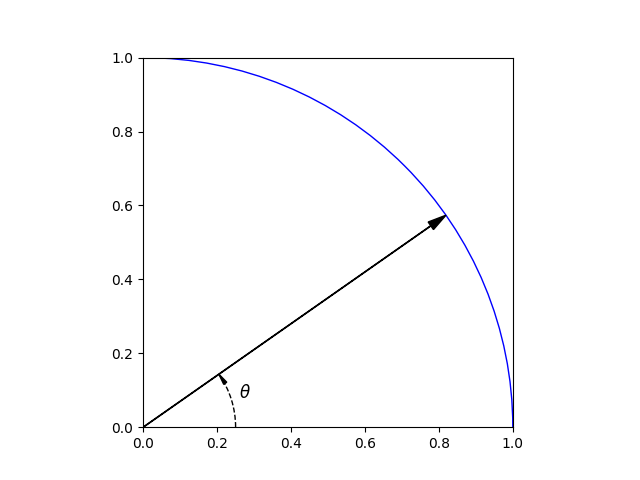
\includegraphics[width=0.6\textwidth]{figures/cad/quarter_circle_polar}
\caption{Quarter of circle of radius 1, using polar coordinates.}
\label{fig:quarter_circle_polar}
\end{figure}

in which case we can compute its derivative as 
\begin{align}
  \mathcal{C}^\prime(\theta) = 
  \begin{bmatrix}
    -\sin \theta \\ \cos \theta
  \end{bmatrix}
  \label{eq:quarter-circle-polair-derivative}
\end{align}
The tangent at $\theta = 0$ and $\theta = \frac{\pi}{2}$ are then given by 
$\mathcal{C}^\prime(\theta := 0) = 
  \begin{bmatrix}
    0 \\ 1 
  \end{bmatrix}
$ 
and 
$\mathcal{C}^\prime(\theta := \frac{\pi}{2}) = 
  \begin{bmatrix}
    -1 \\ 0 
  \end{bmatrix}
$.
\\
\noindent
Another way to represent the quarter of circle, is to introduce the variable $t := \tan \frac{\theta}{2}$, then we get the following rational form \ref{eq:quarter-circle-rational}, where $t \in \left[ 0, 1 \right]$,
\begin{align}
  \mathcal{C}(t) = 
  \begin{bmatrix}
    x(t) \\ y(t)
  \end{bmatrix} =
  \begin{bmatrix}
    \frac{1-t^2}{1+t^2} \\ \frac{2t}{1+t^2}
  \end{bmatrix}
  \label{eq:quarter-circle-rational}
\end{align}

\noindent
There are different advantages for having a parametric form:
\begin{itemize}
  \item Extending a 2D curve to 3D,
  \item Ideal for bounded curves and surfaces,   
  \item Natural orientation of curves and surfaces,
  \item Appropriate representation for design on a computer. In some particular cases, the coefficients in a parametric form possess interesting geometric significance, 
  \item Computing a point on a curve is easy, while finding its parametric value is a in general a non-linear problem, 
\end{itemize}

\begin{remark}
  Notice that in some cases, this representation may introduce singularities that are unrelated to the described geometry.
\end{remark}

\begin{remark}
  Computing the derivatives (tangent or normal vectors at the extremeties) needs an evaluation. We shall be more interested in representation where such informations can be extracted directly from the parametric representations.
\end{remark}

Although one can use any parametric representation for CAD systems, it is important to restrict to a representation that is
\begin{itemize}
  \item capable of reproducing a \textit{wild class} of curves/surfaces
  \item easy to implement
  \item efficient and accurate evaluation 
  \item numerical stable evaluation
  \item \textit{easy} evaluation of points and their derivatives
  \item evaluation complexity of the same or comparable order as polynomials
  \item small memory storage
\end{itemize}

\section{Power basis form of a curve}
If we restrict our representation to polynomials, one naive way would be to use power basis, \textit{i.e.} monomials as in \ref{eq:power-basis-curve}
\begin{align}
  \mathcal{C}(t) = \sum_{i=0}^n \mathbf{a}_i t^i
  \label{eq:power-basis-curve}
\end{align}
where $\mathbf{a}_i = 
\begin{bmatrix}
  a_i^x \\ a_i^y \\ a_i^z
\end{bmatrix}
$ are 2D or 3D vectors.
\\
\noindent
Using the Taylor expansion, we get $\mathcal{C}^\prime(t)|_{t=0} = i! \mathbf{a}_i$, which leads to $\mathbf{a}_i = \frac{\mathcal{C}^\prime(t)|_{t=0}}{i!}$. We then have a direct access to the derivative at $t=0$, but only at this point.
\\
\noindent
The evaluation of such a form can be done using the Horner algorithm as described in \ref{eq:horner-algoritm}:

\begin{align}
  \mathcal{C}(t) = a_0 + t \left( a_1 + t \left( a_2 + t \left( \dots  + t \left( a_{n-1} + t a_{n}    \right)   \right) \right) \right) 
  \label{eq:horner-algoritm}
\end{align}

% ...
\begin{minipage}{\textwidth}
  \begin{algorithm}[H]
  \DontPrintSemicolon
  \SetAlgoLined
  \SetKwInOut{Input}{Input}\SetKwInOut{Output}{Output}
  \Input{$\mathbf{a}, x$}
  \Output{$v$}
  \BlankLine

  $n \gets {\sc len } \left( \mathbf{P} \right) - 1$\;
  $v \gets a[n]$\;
  \For{$i \gets n-1$ \textbf{to} $0$} {
    $v \gets v x + a[i]$\;
  }
  \Return{$v$}\;

  \caption{{\sc Horner}: Evaluation of a polynomial defined by its coefficients $\mathbf{a}$ at $x$.}
  \label{algo:horner}
  \end{algorithm} 
\end{minipage}
% ...

%The Python code \ref{code:horner}, implementations the sequential Horner algorithm.
%
%\begin{code}
%  \centering
%  \begin{python}
%  def horner(a, x):
%      """
%      evaluation of a power basis curve at a point 'x'.
%      'a' contains the coefficients
%      """
%      n = len(a) - 1
%      c = a[n]
%      for i in range(0, n)[::-1]:
%          c = c*x + a[i]
%      return c
%  \end{python}
%  \caption{Python implementation of the sequential Horner algorithm.}
%  \label{code:horner}
%\end{code}

\begin{remark}
  The Horner algorithm is numerically unstable for high degrees, more details can be found in  \cite{FAROUKI1987191} \cite{FAROUKI19881} \cite{HighamBook2002} \cite{Boldo2004}.
\end{remark}

%\todo{add example + exercise + check it using the Python code}

\begin{remark}
  The use of power basis form is not suited for shape and geometric design; the coefficients do not have any geoemtric meaning and modifying them do not allow for a good control of a curve or a surface,  
\end{remark}

% ...................................................................
\section{Problems}
\label{sec:cad-intro-problems}

\begin{exercise}
  Consider the two parametric representations of the circular arc given by Eqs. (\ref{eq:quarter-circle-polair}) and (\ref{eq:quarter-circle-rational}). Using Eq. (\ref{eq:quarter-circle-polair}), compute the curve point at $u = \frac{\pi}{4}$ and, using Eq. (\ref{eq:quarter-circle-rational}), the point at $t = \frac{1}{2}$. Explain the results.
\end{exercise}

\begin{exercise}
  Compute the acceleration vector, $\mathcal{C}^{\prime\prime}(u)$, for Eq. (\ref{eq:quarter-circle-polair}). Explain the result.
\end{exercise}

\begin{exercise}
  Consider the parabolic arc $\mathcal{C}^{\prime\prime}(u) = (x(u), y(u)) = \left( -1-u+2u^2, -2u, u^2 \right)$ for $0 \leq u \leq 1$. Plot the curve $\mathcal{C}$, then apply the transformations
  \begin{itemize}
    \item a rotation of $\frac{\pi}{2}$ about the origin. We recall that the rotation matrix (applied from the left) is 
      \begin{align*}
        \begin{pmatrix}
          0 & -1 \\
          1 &  0
        \end{pmatrix}
      \end{align*}
    \item a translation with the vector $\left( -1, -1 \right)$.
  \end{itemize}
  Compute the implicit equation of the associated parabola.
\end{exercise}

\begin{exercise}
  Determine formulas for the number of additions and multiplications necessary to compute a point on an nth-degree three-dimensional power basis curve.
\end{exercise}

\begin{exercise}
  Construct a cubic power basis curve with a loop. Hint: think about what end- points and end derivatives, $\mathcal{C}^\prime(0)$ and $\mathcal{C}^\prime(1)$, are necessary.
\end{exercise}

\begin{exercise}
Construct a cubic power basis curve with a cusp. Hint: think about $\mathcal{C}^\prime(u)$ and
$\mathcal{C}^{\prime\prime}(u)$. 
Sketch what $x^{\prime}(u), y^{\prime}(u), x^{\prime\prime}(u)$, and $y^{\prime\prime}(u)$ need to look like as functions of $u$.
Determine a suitable $\mathcal{C}^{\prime\prime}(u)$, and then integrate to obtain $\mathcal{C}^\prime(u)$ and $\mathcal{C}(u)$.
\end{exercise}

\begin{exercise}
Construct a cubic power basis curve with an inflection point.
\end{exercise}

\begin{exercise}
  Compare the CPU cost for an evaluation for the presented representations.
  % 60 + 60 for polar case
\end{exercise}

\begin{exercise}
  Compute the CPU cost for the Horner algorithm.
\end{exercise}

\begin{exercise}
  Write a Python implementation for the Horner algorithm.
\end{exercise}

\begin{exercise}[Parallel evaluation]
  Let us consider a polynomial $P$ of degree $n$, defined as $P(t) = \sum_{i=0}^{n} a_i t^i$. Using the form 
  \begin{align*}
   P(t) = \sum_{j=0}^{k-1} x^j P_j(x^k) 
  \end{align*}
  as a splitting into $k$ independent parts, write a Python code for the parallel evaluation and compute its complexity.
\end{exercise}


% *********** chapter1.tex
\chapter{B\'ezier curves}
%\minitoc
\label{ch:cad-bezier}
\section{Bernstein polynomials}
In 1885, Weierstrass proved that the set of polynomial functions on $\left[0, 1\right]$ is dense in $\mathcal{C}\left( \left[0, 1\right] \right)$. In 1912, Sergei Bernstein gave a simple proof to this result by introducing the now-famous Bernstein polynomials \ref{eq:bernstein}:

\begin{align}
  B_k^n (x) =  \binom{n}{k} x^k (1-x)^{n-k}, \quad \mbox{where}\quad k \in \left[0, n \right] ~ \mbox{and} ~ x \in \left[ 0, 1 \right]
  \label{eq:bernstein}
\end{align}
\noindent
In figure Fig. \ref{fig:bernstein}, we plot Bernstein polynomials of degrees $1$ to $5$. From these plots, we see that Bernstein polynomials are positive, the first and last polynomials are equal to $1$ on the $0$ and $1$ respectivaly. More properties will be discussed in the sequel.

%
\begin{figure}[ht!]
\centering
\begin{minipage}[t]{0.43\textwidth}
  \centering
  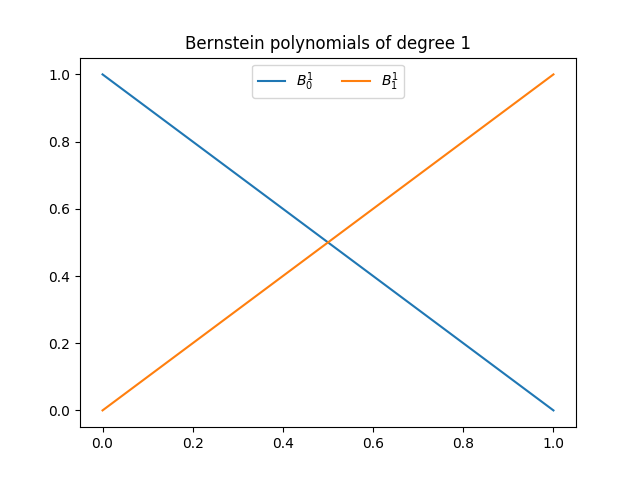
\includegraphics[width=1.0\textwidth]{figures/cad/all_bernstein_degree_1}
\end{minipage}
\begin{minipage}[t]{0.43\textwidth}
  \centering
  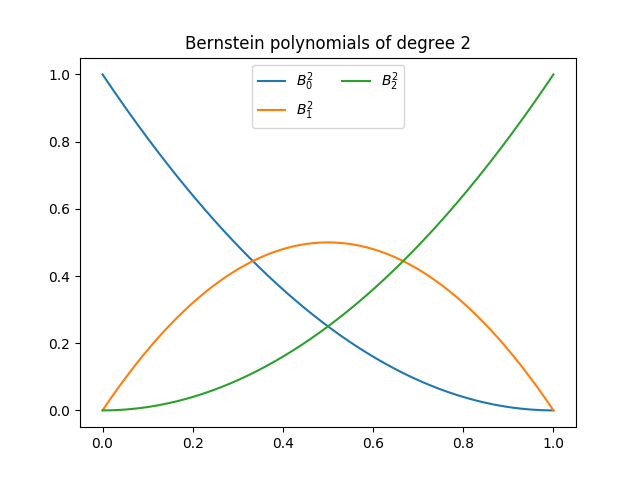
\includegraphics[width=1.0\textwidth]{figures/cad/all_bernstein_degree_2}
\end{minipage}
\begin{minipage}[t]{0.43\textwidth}
  \centering
  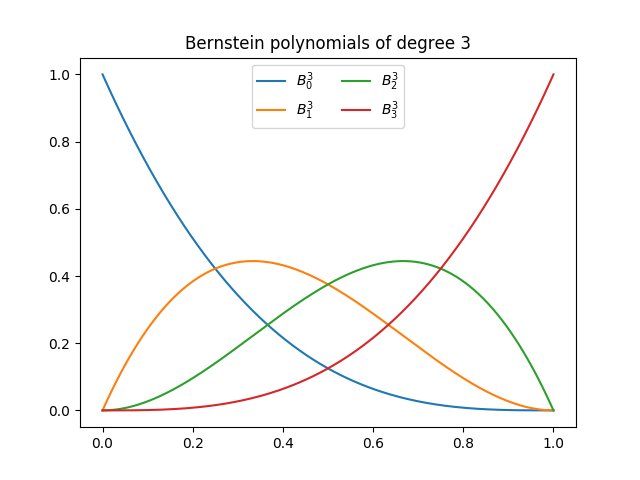
\includegraphics[width=1.0\textwidth]{figures/cad/all_bernstein_degree_3}
\end{minipage}
\begin{minipage}[t]{0.43\textwidth}
  \centering
  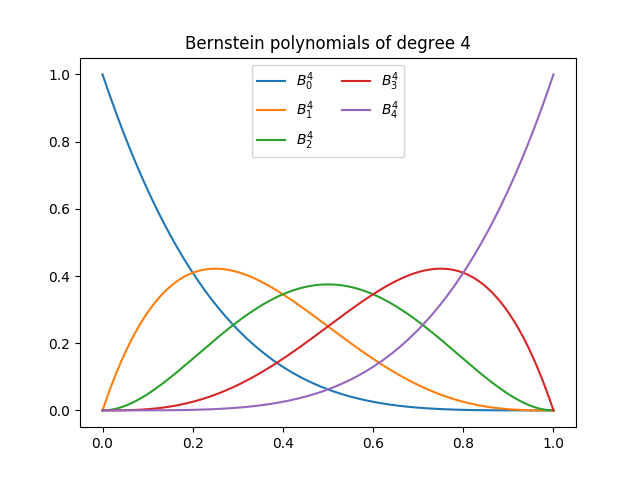
\includegraphics[width=1.0\textwidth]{figures/cad/all_bernstein_degree_4}
\end{minipage}
\begin{minipage}[t]{0.43\textwidth}
  \centering
  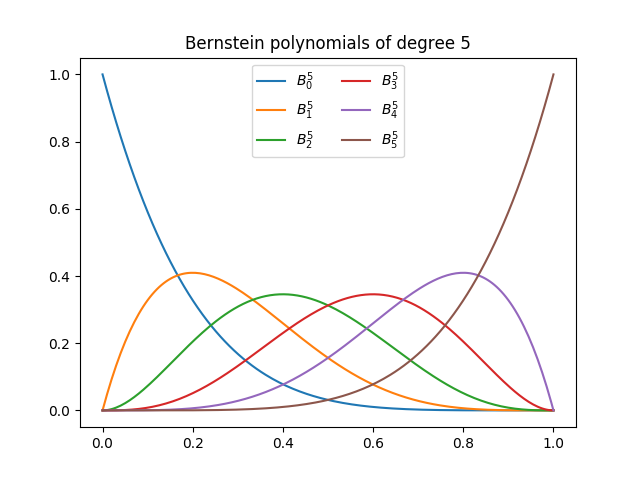
\includegraphics[width=1.0\textwidth]{figures/cad/all_bernstein_degree_5}
\end{minipage}
\caption{Bernstein polynomials of degree $n = 1, 2, 3, 4, 5$.}
  \label{fig:bernstein}
\end{figure}

%%%%%%%%%%%%%%%%%%%%%%
%%  dot2tex bernstein.dot -tmath --figonly > bernstein.tex
%\input{cad/dot/bernstein}
%%%%%%%%%%%%%%%%%%%%%%



\subsubsection*{Properties of Bernstein polynomials}
\begin{itemize}
  \item $B_k^n(x) \ge 0$, for all $k \in \left[0, n \right]$ and $x \in \left[ 0, 1 \right]$ \hfill [positivity] 
  \item $\sum_{k=0}^n B_k^n(x) = 1$, for all $x \in \left[ 0, 1 \right]$ \hfill [partition of unity] 
  \item $B_0^n(0) = B_n^n(1) = 1$ 
  \item $B_k^n$ has exactly one maximum on the interval $\left[ 0, 1 \right]$, at $\frac{k}{n}$ 
  \item $\left( B_k^n(x) \right)_{0 \le k \le n}$ is symmetric with respect to $x = \frac{1}{2}$ \hfill [symmetry]
  \item Bernstein polynomials can be defined recursively using the formulae \ref{eq:bernstein-rec}
    \begin{align}
      B_k^n(x) = (1-x) B_k^{n-1}(x) + x B_{k-1}^{n-1}(x)
      \label{eq:bernstein-rec}
    \end{align}
    where we assume $B_k^n(x) = 0$ is $k < 0$ or $k > n$

    \begin{figure}
    \centering
    \includegraphics[width=0.6\textwidth]{figures/cad/diagrams/bernstein}
    \caption{General evaluation triangular diagram for a Bernstein polynomials.}
    \label{fig:bernstein-triangular-diagram}
    \end{figure}

  \item Bernstein derivatives can be computed using the formulae \ref{eq:bernstein-der} 
    \begin{align}
      {B_k^n}^\prime(x) = n \left(B_{k-1}^{n-1}(x) - B_k^{n-1}(x) \right)
      \label{eq:bernstein-der}
    \end{align}
    using the same assumption as before.
\end{itemize}

%\subsubsection*{Evaluation of Bernstein polynomials}
% TODO move to Jupyter Notebooks
%In this section, we shall see different algorithms to evaluate Bernstein polynomials of a given degree. We first start by the naive implementation given in Code. \ref{code:bernstein_v1}. We see that for every evaluation, we must perform $n$ multiplications to compute the terms in $x$ and $1-x$, while the evaluation of the binomial coefficient takes $n$ multplications and $1$ division. This is clearly not optimal.
%
%\begin{code}
%  \centering
%  \begin{python}
%  from scipy.special import binom
%
%  def bernstein_v1(n,k,x):
%      return binom(n,k) * x**k * (1.-x)**(n-k)
%  \end{python}
%  \caption{Naive implementation for the evaluation of Bernstein polynomials}
%  \label{code:bernstein_v1}
%\end{code}
%
%\begin{code}[ht!]
%\centering
%  \begin{python}
%  def bernstein_v2(n,k,x):
%      if k < 0 or k > n: return 0.
%      if n == 0: return 1.
%      return (1.-x)*bernstein_v2(n-1,k,x) + x*bernstein_v2(n-1,k-1,x)
%  \end{python}
%  \caption{Reccursive implementation for the evaluation of Bernstein polynomials}
%  \label{code:bernstein_v2}
%\end{code}
%
%\begin{code}[ht!]
%\centering
%  \begin{python}
%  from functools import lru_cache
%
%  @lru_cache(maxsize=None)
%  def bernstein_v3(n,k,x):
%      if k < 0 or k > n: return 0.
%      if n == 0: return 1.
%      return (1.-x)*bernstein_v2(n-1,k,x) + x*bernstein_v2(n-1,k-1,x)
%  \end{python}
%  \caption{Reccursive implementation for the evaluation of Bernstein polynomials using \texttt{LRU\_CACHE} decorator in Python, to save all the recent calls.}
%  \label{code:bernstein_v3}
%\end{code}
%
%
%\begin{code}[ht!]
%\centering
%  \begin{python}
%  import numpy as np
%
%  def bernstein_v4(n,k,x):
%      tmp = np.zeros(n+1)
%      tmp[n-k] = 1.
%      x1 = 1.-x
%      for i in range(1, n+1):
%          for j in range(i, n+1)[::-1]:
%              tmp[j] = x1*tmp[j] + x*tmp[j-1]
%      return tmp[n]
%  \end{python}
%  \caption{Naive implementation for the evaluation of Bernstein polynomials}
%  \label{code:bernstein_v4}
%\end{code}
%
%\begin{code}[ht!]
%\centering
%  \begin{python}
%  import numpy as np
%
%  def bernstein_v5(n,k,x,tmp):
%      tmp[:] = 0.
%      tmp[n-k] = 1.
%      x1 = 1.-x
%      for i in range(1, n+1):
%          for j in range(i, n+1)[::-1]:
%              tmp[j] = x1*tmp[j] + x*tmp[j-1]
%      return tmp[n]
%  \end{python}
%  \caption{Naive implementation for the evaluation of Bernstein polynomials}
%  \label{code:bernstein_v5}
%\end{code}
%
%\begin{code}[ht!]
%\centering
%  \begin{python}
%  import numpy as np
%
%  def all_bernstein(n, x):
%      b = np.zeros(n+1)
%      b[0] = 1.
%      x1 = 1.-x
%      for j in range(1, n+1):
%          saved = 0.
%          for i in range(0, j):
%              tmp = b[i]
%              b[i] = saved + x1*tmp
%              saved = x*tmp
%          b[j] = saved
%      return b
%  \end{python}
%  \caption{Evaluation of all Bernstein polynomials}
%  \label{code:all_bernstein}
%\end{code}
%
%
%
%\clearpage
\section{B\'ezier curves}
Rather than taking the power basis as in \ref{eq:power-basis-curve}, Pierre B\'ezier used Bernstein polynomials, in the 1960s while working at \textit{Renault}. This leads to the following definition of a polynomial curve \ref{eq:bezier-curve}

\begin{align}
  \mathcal{C}(t) = \sum_{k=0}^n \mathbf{P}_k B_k^n(t) 
  \label{eq:bezier-curve}
\end{align}
\noindent
The vector coefficients $\left( \mathbf{P} \right)_{0 \le k \le n}$ are called \textit{B\'ezier points} or \textbf{control points}. The reason for this will become clear in the sequel.

\subsubsection*{Examples}
\begin{description}
  \item[\textbf{Example 1.}] A linear ($n=1$) B\'ezier curve (fig. \ref{fig:bezier-ex1}) is defined as 
    $$\mathcal{C}(t) = \mathbf{P}_0 B_0^1(t) + \mathbf{P}_1 B_1^1(t)$$ 
    which describes a straight line from $\mathbf{P}_0$ to $\mathbf{P}_1$, since $B_0^1(t) = 1-t$ and $B_1^1(t) = t$. 

  \begin{figure}
  \centering
  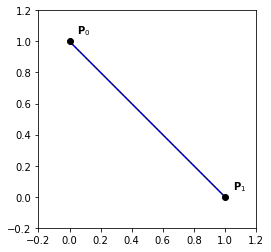
\includegraphics[width=.6\textwidth]{figures/cad/bezier/ex1}
  \caption{Example of a linear B\'ezier curve.}
  \label{fig:bezier-ex1}
  \end{figure}

  \item[\textbf{Example 2.}] A quadratic ($n=2$) B\'ezier curve (fig. \ref{fig:bezier-ex2}) is defined as 
    $$\mathcal{C}(t) = (1-t)^2 \mathbf{P}_0  + 2t(1-t) \mathbf{P}_1 + t^2 \mathbf{P}_2$$  

  \begin{figure}
  \centering
  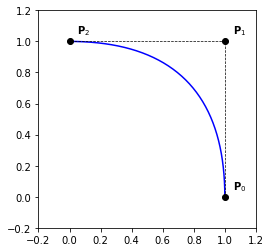
\includegraphics[width=.6\textwidth]{figures/cad/bezier/ex2}
  \caption{Example of a quadratic B\'ezier curve.}
  \label{fig:bezier-ex2}
  \end{figure}

  We remark that
  \begin{itemize}
    \item[-] the curve starts at $\mathbf{P}_{0}$ and  ends at $\mathbf{P}_{2}$,
    \item[-] the curve does not pass through the point $\mathbf{P}_{1}$,
    \item[-] the tangent directions to the curves at its extremeties are parallel to $\mathbf{P}_{1} - \mathbf{P}_{0}$ and $\mathbf{P}_{2} - \mathbf{P}_{1}$,
    \item[-] the curve is contained in the polygone (triangle) formed by $\mathbf{P}_{0}\mathbf{P}_{1}\mathbf{P}_{2}$. This polygone is called the \textit{control polygon} and it approximates the shape of the curve.
  \end{itemize}

  \item[\textbf{Example 3.}] A cubic ($n=3$) B\'ezier curve (figures \ref{fig:bezier-ex3a},\ref{fig:bezier-ex3b},\ref{fig:bezier-ex3c}) is defined as 
    $$\mathcal{C}(t) = (1-t)^3 \mathbf{P}_0  + 3t(1-t)^2 \mathbf{P}_1 + 3t^2(1-t) \mathbf{P}_2 + t^3 \mathbf{P}_3$$  

  \begin{figure}
  \centering
  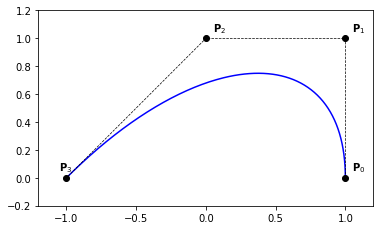
\includegraphics[width=.6\textwidth]{figures/cad/bezier/ex3a}
  \caption{Example of a cubic B\'ezier curve.}
  \label{fig:bezier-ex3a}
  \end{figure}

  \begin{figure}
  \centering
  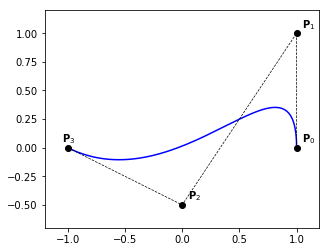
\includegraphics[width=.6\textwidth]{figures/cad/bezier/ex3b}
  \caption{Example of a cubic B\'ezier curve.}
  \label{fig:bezier-ex3b}
  \end{figure}

  \begin{figure}
  \centering
  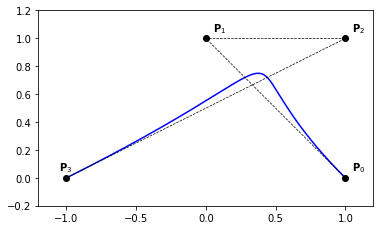
\includegraphics[width=.6\textwidth]{figures/cad/bezier/ex3c}
  \caption{Example of a cubic B\'ezier curve.}
  \label{fig:bezier-ex3c}
  \end{figure}

  We remark that
  \begin{itemize}
    \item[-] the curves start at $\mathbf{P}_{0}$ and end at $\mathbf{P}_{3}$,
    \item[-] the curves do not pass through the points $\mathbf{P}_{1}$ and $\mathbf{P}_{2}$,
    \item[-] the tangents directions to the curves at their extremeties are parallel to $\mathbf{P}_{1} - \mathbf{P}_{0}$ and $\mathbf{P}_{3} - \mathbf{P}_{2}$,
    \item[-] the control polygons approximate the shape of the curves,
    \item[-] the curves follow the orientation of the control polygons,
    \item[-] the curves are contained in the convex hulls of their control polygons (\textit{convex hull property}).
  \end{itemize}

\end{description}


%\begin{figure}[ht!]
%\centering
%\begin{minipage}[t]{1.0\textwidth}
%\begin{python}[caption={TODO},captionpos=b, label={code:point_bezier_curve}]
%def point_on_bezier_curve(P,x):
%    n = len(P) - 1
%    b = all_bernstein(n, x)
%    c = 0.
%    for k in range(0, n+1):
%        c += b[k]*P[k]
%    return c
%\end{python}
%\end{minipage}
%\end{figure}

%\todo{add remarks p22}

\subsubsection*{Derivatives of a B\'ezier curve}
\noindent
Using the formulae \ref{eq:bernstein-der}, we have
\begin{align*}
  \mathcal{C}^\prime(t) = \sum_{k=0}^n \mathbf{P}_k {B_k^n}^\prime(t) 
                        = \sum_{k=0}^n n \mathbf{P}_k \left(B_{k-1}^{n-1}(x) - B_k^{n-1}(x) \right)  
\end{align*}
by reordering the indices, we get \ref{eq:bezier-curve-der}
\begin{align}
  \mathcal{C}^\prime(t) &= \sum_{k=0}^{n-1} n \left( \mathbf{P}_{k+1} - \mathbf{P}_k \right) B_k^{n-1}(t) 
  \label{eq:bezier-curve-der}
\end{align}
Therefor, we get the direct acces to the first order derivatives at the extremeties of a B\'ezier curve using the formulae \ref{eq:bezier-curve-der-1-ext}

\begin{align}
  \begin{cases}
    \mathcal{C}^\prime(0) = n \left( \mathbf{P}_{1} - \mathbf{P}_0 \right)  
    \\ 
    \mathcal{C}^\prime(1) = n \left( \mathbf{P}_{n} - \mathbf{P}_{n-1} \right)  
  \end{cases}
  \label{eq:bezier-curve-der-1-ext}
\end{align}
\noindent
Second derivatives can also be computed directly from the control points using the formulae  \ref{eq:bezier-curve-der-2-ext}

\begin{align}
  \begin{cases}
    \mathcal{C}^{\prime\prime}(0) = n(n-1) \left( \mathbf{P}_{0} - 2 \mathbf{P}_1 + \mathbf{P}_{2} \right)  
    \\ 
    \mathcal{C}^{\prime\prime}(1) = n(n-1) \left( \mathbf{P}_{n} - 2 \mathbf{P}_{n-1} + \mathbf{P}_{n-2} \right)  
  \end{cases}
  \label{eq:bezier-curve-der-2-ext}
\end{align}

%\todo{add formulae for higher derivatives}
%\todo{Explain why the control points are called so}

\begin{definition}[$r^{th}$ forward difference]
  Let us consider a set of (control) points $\mathbf{P}$.
  The $r^{th}$ forward difference of $\mathbf{P}$ is defined as  
  \begin{align*}
    \triangle^r \mathbf{P}_i := \triangle^{r-1} \mathbf{P}_{i+1} - \triangle^{r-1} \mathbf{P}_i  
  \end{align*}
  with 
  \begin{align*}
    \triangle \mathbf{P}_i = \triangle^1 \mathbf{P}_i := \mathbf{P}_{i+1} - \mathbf{P}_i  
  \end{align*}
\end{definition}

\begin{proposition}[High order dirivatives]
  \begin{align}
    \mathcal{C}^{(r)}(t) = \frac{n!}{\left( n-r \right)!} \sum\limits_{i=0}^{n-r} \triangle^r \mathbf{P}_i B_i^{n-r}(t) 
    \label{eq:bezier-high-deriv}
  \end{align}
\end{proposition}
\noindent
Eqs (\ref{eq:bezier-curve-der-1-ext}) and (\ref{eq:bezier-curve-der-2-ext}) can be generelaized for high order derivatives. We have in fact the following result:
\begin{remark}
The derivatives of a B\'ezier curve at its extremeties up to order $r$ depend only on the first (or last) $r+1$ control points, and vice versa.
\end{remark}
\begin{proposition}
  \label{prop:bezier-forward-difference}
  $$\triangle^r \mathbf{P}_0 = \sum\limits_{i=0}^{r} \left( -1 \right)^{r-i} \binom{r}{i} \mathbf{P}_i $$
\end{proposition}

\subsubsection*{Integration of B\'ezier curves}
\begin{proposition}
A primitive of A B\'ezier curve $\mathcal{C}(t) = \sum_{k=0}^n \mathbf{P}_k B_k^n(t)$ has the B\'ezier representation
\begin{align}
  \left( \int \mathcal{C} \right) (t) = \sum_{k=0}^{n+1} \mathbf{Q}_k B_k^{n+1}(t)
  \label{eq:bezier-primitive}
\end{align}
where
\begin{align*}
  \mathbf{Q}_k := \mathbf{Q}_{k-1} + \frac{1}{n+1} \mathbf{P}_{k-1} 
                = \mathbf{Q}_{0}  + \frac{1}{n+1} \left( \sum\limits_{i=0}^{k-1} \mathbf{P}_{i}  \right)
\end{align*}
\end{proposition}
Here, $\mathbf{Q}_{0}$ denotes an arbitrary integration constant.
\begin{remark}
  Using Eq. (\ref{eq:bezier-primitive}), we have $\int_0^1 \mathcal{C}(t)~dt = \frac{1}{n+1}\left( \sum\limits_{i=0}^n \mathbf{P}_i \right)$.
\end{remark}

\subsubsection*{Properties of B\'ezier curves}
Because of the \textit{symmetry} of the Bernstein polynomials, we have
\begin{itemize}
  \item  $\sum_{k=0}^n \mathbf{P}_k B_k^n = \sum_{k=0}^n \mathbf{P}_k B_{n-k}^n $
\end{itemize}
Thanks to the interpolation property, for $B_0^n$ and $B_n^n$, of the Bernstein polynomials at the endpoints, we get
\begin{itemize}
  \item $\mathcal{C}(0) = \mathbf{P}_0$  and $\mathcal{C}(1) = \mathbf{P}_n$ 
\end{itemize}
Using the partition unity property of the Bernstein polynomials, we get
\begin{itemize}
  \item any point $\mathcal{C}(t)$ is an \textit{affine combination} of the control points 
\end{itemize}
Therefor,
\begin{itemize}
  \item B\'ezier curves are affinely invariant; \textit{i.e.} the image curve $\Phi(\sum_{k=0}^n \mathbf{P}_k B_k^n)$ of a B\'ezier curve, by an affine mapping $\Phi$, is the B\'ezier curve having $\left( \Phi(\mathbf{P}_i) \right)_{0 \le i \le n}$ as control points. 
\end{itemize}
due to the partition unity of the Bernstein polynomials and their non-negativity, 
\begin{itemize}
  \item any point $\mathcal{C}(t)$ is a \textit{convex combination} of the control points 
\end{itemize}
finally, we get the \textit{convex hull property},
\begin{itemize}
  \item A B\'ezier curve lies in the convex hull of its control points 
\end{itemize}

\section{DeCasteljau Algorithm}
In this section, we introduce the deCasteljau algorithm Algo. (\ref{algo:decasteljau}). The basic idea comes from the following remark;
using the reccurence formulae Eq. (\ref{eq:bernstein-rec}), we have
\begin{align*}
  \mathcal{C}(t) &= \sum_{k=0}^n \mathbf{P}_k B_k^n(t) = \sum_{k=0}^n \mathbf{P}_k \left( (1-t) B_k^{n-1}(t) + t B_{k-1}^{n-1}(t) \right) \\ 
                 &= \sum_{k=0}^{n-1} \mathbf{P}_k^1  B_k^{n-1}(t) \quad\quad\quad\quad\quad [\mathbf{P}_k^{1} := (1-t)\mathbf{P}_k + t \mathbf{P}_{k+1}] \\ 
                 &= \sum_{k=0}^{n-2} \mathbf{P}_k^2  B_k^{n-2}(t) \quad\quad\quad\quad\quad [\mathbf{P}_k^{2} := (1-t)\mathbf{P}_k^1 + t \mathbf{P}_{k+1}^1] \\ 
                 &= \ldots \\
                 &= \sum_{k=0}^{0} \mathbf{P}_k^n  B_k^{0}(t) \quad\quad\quad\quad\quad [\mathbf{P}_k^{n} := (1-t)\mathbf{P}_k^{n-1} + t \mathbf{P}_{k+1}^{n-1}] \\ 
                 &= \mathbf{P}_0^n 
\end{align*}
% ...
\begin{minipage}{\textwidth}
  \begin{algorithm}[H]
  \DontPrintSemicolon
  \SetAlgoLined
  \SetKwInOut{Input}{Input}\SetKwInOut{Output}{Output}
  \Input{$\mathbf{P}, x$}
  \Output{$value$}
  \BlankLine

  $n \gets {\sc len } \left( \mathbf{P} \right) - 1$\;
  $\mathbf{Q} \gets \mathbf{P}$\;
  \For{$j \gets 0$ \textbf{to} $n$} {
    \For{$i \gets 0$ \textbf{to} $n-j$} {
      $Q[i] \gets (1-x) Q[i] + x Q[i+1]$\;
    }
  }
  \Return{$Q[0]$}\;

  \caption{{\sc DeCasteljau}: Evaluation of a B\'ezier curve, defined by its control points $\mathbf{P}$ at $x$.}
  \label{algo:decasteljau}
  \end{algorithm} 
\end{minipage}
% ...

\section{Conversion from/to monomial form}
\subsubsection*{Conversion from monomial form}
Let us consider a monomial representation of a curve 
\begin{align*}
\mathcal{C}(t) = \sum_{k=0}^n \mathbf{Q}_k t^k 
\end{align*}
Since
\begin{align*}
  t^k &= \frac{1}{\binom{n}{k}} \binom{n}{k} t^k \left(1-t+t \right)^{n-k} 
      = \frac{1}{\binom{n}{k}} \left( \sum\limits_{i=0}^{n-k} \binom{n}{k} \binom{n-k}{n-k-i} t^{i+k} \left( 1-t \right)^{n-k-i} \right) \\
      &= \frac{1}{\binom{n}{k}} \left(  \sum\limits_{i=0}^{n-k} \binom{k+i}{k} B_{k+i}^n(t) \right)
      = \frac{1}{\binom{n}{k}} \left(  \sum\limits_{j=0}^{n} \binom{j}{k} B_{j}^n(t) \right) 
\end{align*}
we get,
\begin{align*}
\mathcal{C}(t) = \sum_{k=0}^n \mathbf{Q}_k t^k = \sum_{k=0}^n \mathbf{Q}_k \frac{1}{\binom{n}{k}} \left(  \sum\limits_{j=0}^{n} \binom{j}{k} B_{j}^n(t) \right)  
\end{align*}
hence,
\begin{align*}
\mathcal{C}(t) = \sum_{j=0}^n \left(\sum\limits_{k=0}^{n} \frac{\binom{j}{k}}{\binom{n}{k}} \mathbf{Q}_k \right) B_{j}^n(t)  
\end{align*}
which is a B\'ezier curve of the form
\begin{align*}
\mathcal{C}(t) = \sum_{k=0}^n \mathbf{P}_k B_k^n(t)
\end{align*}
with 
\begin{align*}
\mathbf{P}_k =  \sum\limits_{k=0}^{n} \frac{\binom{j}{k}}{\binom{n}{k}} \mathbf{Q}_k 
\end{align*}
\begin{remark}
  If $\mathbf{Q}_k = 0$ for all $k \geq 2$, then the control points are given by $\mathbf{P}_k = \mathbf{Q}_0 + k \mathbf{Q}_1$.
\end{remark}
\begin{proposition}[Linear Precision]
  Conversly, if the $n+1$ control points $\mathbf{P}$ lie equidistantly on a line, then $\mathcal{C}$ is a linear polynomial, which can be written as $\mathcal{C}(t) = \left(1-t\right) \mathbf{P}_0 + t \mathbf{P}_n$. 
\end{proposition}
\subsubsection*{Conversion to monomial form}
Given a B\'ezier curve $\mathcal{C}(t) = \sum_{k=0}^n \mathbf{P}_k B_k^n(t)$, we can derive its monomial representation using the Taylor expansion,
\begin{align*}
  \mathcal{C}(t) &= \sum\limits_{k=0}^n \frac{1}{k!}\mathcal{C}^{(k)}(0) t^k \\
                 &= \sum\limits_{k=0}^n \binom{n}{k} \triangle^k \mathbf{P}_0 t^k  
\end{align*}

\section{Rational B\'ezier curves}
We first introduce the notion of Rational Bernstein polynomials defined as,  and $w_i > 0, \forall i \in \left[0, n \right]$ 
\begin{align}
  R_k^n(t) := \frac{w_i B_k^n(t)}{\sum_{i=0}^n w_i B_i^n(t)}
  \label{eq:rational-bernstein}
\end{align}

\subsubsection*{Properties of Rational Bernstein polynomials}
\begin{itemize}
  \item $R_k^n(x) \ge 0$, for all $k \in \left[0, n \right]$ and $x \in \left[ 0, 1 \right]$ \hfill [positivity] 
  \item $\sum_{k=0}^n R_k^n(x) = 1$, for all $x \in \left[ 0, 1 \right]$ \hfill [partition of unity] 
  \item $R_0^n(0) = R_n^n(1) = 1$ 
  \item $R_k^n$ has exactly one maximum on the interval $\left[ 0, 1 \right]$, 
  \item Bernstein polynomials are Rational Bernstein polynomials when all weights are equal
\end{itemize}

\begin{definition}[Rational B\'ezier curve]

\begin{align}
  \mathcal{C}(t) = \sum_{k=0}^n \mathbf{P}_k R_k^n(t) 
  \label{eq:bezier-curve}
\end{align}

where $R_k^n(t) := \frac{w_i B_k^n(t)}{\sum_{i=0}^n w_i B_i^n(t)}$ and $w_i > 0, \forall i \in \left[0, n \right]$ 
  
\end{definition}

\subsubsection*{Examples}
\begin{description}
  \item[\textbf{Example 1.}] We consider the quadratic Rational B\'ezier curve, 

    \begin{figure}
    \centering
    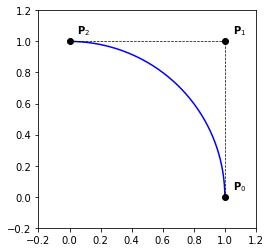
\includegraphics[width=.6\textwidth]{figures/cad/bezier/rational_ex1}
    \caption{Circular arc using quadratic Rational B\'ezier curve.}
    \label{fig:bezier-rational-ex1}
    \end{figure}

    where the weights are given by $w_0 = 1$, $w_1=1$ and $w_2=2$ and the control points are 
    $\mathbf{P}_0 = \begin{pmatrix} 1 \\ 0 \end{pmatrix}$,
    $\mathbf{P}_1 = \begin{pmatrix} 1 \\ 1 \end{pmatrix}$ and
    $\mathbf{P}_2 = \begin{pmatrix} 0 \\ 1 \end{pmatrix}$.
    \\
    This leads to a representation of the circular arc, using the parametric form $\mathcal{C}(t) = \begin{pmatrix} \frac{1-t^2}{1+t^2} \\ \frac{2t}{1+t^2} \end{pmatrix}$.
\end{description}


\section{Composite B\'ezier curves}
A composite B\'ezier curve is a piecewise B\'ezier curve that is at least continuous at the interpolant control points. An example is given in Fig. \ref{fig:composite-bezier-curve}. The global curve inherit all the nice properties of B\'ezier curves however, it has a major drawback: when moving an interpolant control point, we must ensure that the associated regularity is not broken, unless it is what we want. This means that a good representation of a curve needs to have the locality control through control points, but also the control points must be associated to some given regularity. 
\begin{figure}
  \centering
  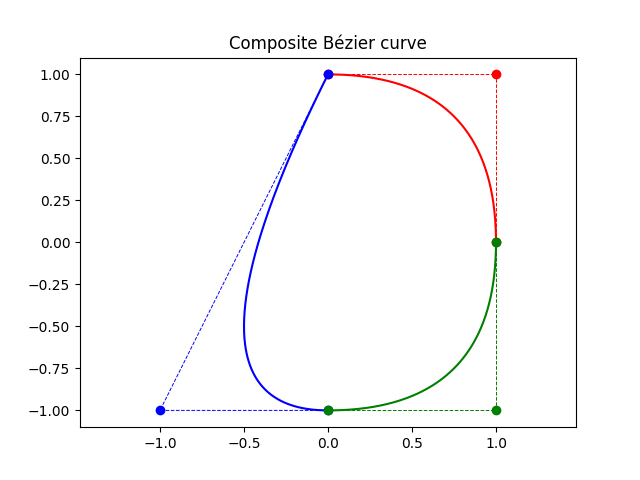
\includegraphics[width=0.6\textwidth]{figures/cad/composite_bezier_curve}
\caption{A composite B\'ezier curve using 3 quadratic B\'ezier curves.}
\label{fig:composite-bezier-curve}
\end{figure}
\noindent
Since Bernstein polynomials are defined locally on the interval $\left[ 0, 1 \right]$, and they do not encode any global redularity of the curve, we need another representation, in terms of other functions, while keeping in mind that these functions must be polynomials on every sub-interval. Such representation is provided by the Schoenberg spaces, for which B-Splines form a basis. In the next chapter, we will first introduce the uniform Splines, also known as Cardinal Splines, show their advantages and limitations, then we will introduce the general definition of B-Splines.



%\section{B\'ezier surfaces}
%\todo{TODO}


%%%%%%%%%%%%%%%%%%%%%%%%%%%%%%%%%%%%%%%%%%%


%\todo{Talk about Gibbs phenomena}

% ...................................................................


\section{Problems}
\label{sec:cad-bezier-problems}

\begin{exercise}
  Show all Bernstein properties.
\end{exercise}

\begin{exercise}
  Consider a cubic B\'ezier curve $\mathcal{C}$ in $\mathbb{R}^2$ with th following control points:
  \begin{align*}
    \mathbf{P}_0 = \left(0, 6 \right), \quad
    \mathbf{P}_1 = \left(3, 6 \right), \quad
    \mathbf{P}_2 = \left(6, 3 \right), \quad
    \mathbf{P}_3 = \left(6, 0 \right)
  \end{align*}
  Compute the point $\mathcal{C}(\frac{1}{3})$ using the deCasteljau algorithm. Compute the same point by Eqs. (\ref{TODO}) and (\ref{TODO}), meaning, evaluate the basis functions at $u=\frac{1}{3}$ then multiply by the associated control points.
\end{exercise}

\begin{exercise}
  The Bernstein operator $\mathcal{B}$ assigns to a function $f$ on $[0,1]$ the polynomial
  \begin{align*}
    \mathcal{B}[f](t) := \sum\limits_{i=0}^n f(\frac{i}{n}) B_i^n(t)
  \end{align*}
  Show that if $f$ is a polynomial of degree $m \leq n$, then $\mathcal{B}[f]$ is also a polynomial of degree $m$.
\end{exercise}

\begin{exercise}
  Show that a planar cubic B\'ezier curve has a cusp if $\mathbf{P}_3$ lies on the parabola
  \begin{align*}
    t \rightarrow \left( \mathbf{P}_0 + \mathbf{P}_1 - \mathbf{P}_2 \right) B_0^2(t) + \mathbf{P}_1 B_1^2(t) + \mathbf{P}_2 B_2^2(t)    
  \end{align*}
\end{exercise}

\begin{exercise}
  For which choices of $\mathbf{P}_3 $ does a planar cubic B\'ezier curve have a loop?
\end{exercise}

\begin{exercise}
  We consider a B\'ezier curve $\mathcal{C}(t) = \sum_{k=0}^n \mathbf{P}_k B_k^n(t)$. 
  \\
  \begin{enumerate}
    \item  Show that using the definition of Bernstein polynomials, we can write $\mathcal{C}$ as
      \begin{align*}
        \mathcal{C}(t) = \left( 1-t \right)^n \left( \sum\limits_{i=0}^n \mathbf{P}_k \binom{n}{k} \left( \frac{t}{1-t} \right)^k \right)
      \end{align*}
    \item Write a modifier version of Horner algorithm based on the previous formula and compute its arithmetic complexity. 
    \item What happens when $t$ is close to $1$? How to adapt the previous algorithm in this case? 
  \end{enumerate}
\end{exercise}

\begin{exercise}
  .
\end{exercise}

\begin{exercise}
  .
\end{exercise}

\begin{exercise}
  .
\end{exercise}

\begin{exercise}
  .
\end{exercise}

\begin{exercise}
  .
\end{exercise}

\begin{exercise}
  .
\end{exercise}




% *********** historical_notes.tex
\chapter{Historical Notes}
\label{ch:cad-historical-notes}

References: \cite{PieglBook1996}, \cite{DeBoor_Book2001}, \cite{farin2002curves, farin1999nurbs, prautzsch2002bezier,rogers2001introduction,cohen2001geometric}




%----------------------------------------------------------------------------------------
%	PART 2: Approximation theory for B-Splines 
%----------------------------------------------------------------------------------------
\part{Approximation theory for B-Splines}

% *********** chapter0.tex
\chapter{Divided differences}
\label{ch:approximation-divided}
\section{Lagrange interpolation}
%For more details on this subject we refer to the books of De-Boor \cite{deboor} (for computational aspect), DeVore and Lorentz \cite{devore_book}, and Schumaker \cite{Schumaker1981a} (for more theoretical aspects).
\noindent
Let us consider the interpolation problem for a function $f$ on a given set of (distinct) points $\{ x_0, \cdots,x_n\}$. It is well known that the Lagrange interpolating polynomial of degree $n$ writes
\begin{align}
  p(x; x_0, \ldots, x_n) = \sum\limits_{i=0}^n f(x_i) L_i(x), \quad \mbox{where}~ L_i(x) = \prod\limits_{\underset{j \neq i}{j=0}}^n \frac{x-x_j}{x_i-x_j}, ~~ i = 0, \ldots, n
  \label{eq:lagrange-interpolation}
\end{align}
The evaluation of the Lagrange interpolator can be done with different methods. The standard one is known as \textbf{Aitken method}. Assume we want to interpolate a function $f$ on the points $\{ x_0, \cdots, x_3 \}$. We start by computing:

\begin{align*}
  p(x; x_0, x_1) &= \frac{1}{x_1-x_0} \begin{vmatrix}f(x_0) & x_0 - x \\ f(x_1) & x_1 - x \end{vmatrix}
  \\
  p(x; x_0, x_2) &= \frac{1}{x_2-x_0} \begin{vmatrix}f(x_0) & x_0 - x \\ f(x_2) & x_2 - x \end{vmatrix}
  \\
  p(x; x_0, x_3) &= \frac{1}{x_3-x_0} \begin{vmatrix}f(x_0) & x_0 - x \\ f(x_3) & x_3 - x \end{vmatrix}
  \\
  p(x; x_0, x_1, x_3) &= \frac{1}{x_3-x_1} \begin{vmatrix}p(x; x_0, x_1) & x_1 - x \\ p(x; x_0, x_3) & x_3 - x \end{vmatrix}
  \\
  p(x; x_0, x_1, x_2) &= \frac{1}{x_2-x_1} \begin{vmatrix}p(x; x_0, x_1) & x_1 - x \\ p(x; x_0, x_2) & x_2 - x \end{vmatrix}
\end{align*}
Then the value of the interpolation polynomial of degree $3$ at $x$ is given by

\begin{align*}
  p(x; x_0, x_1, x_2, x_3) &= \frac{1}{x_3-x_2} \begin{vmatrix}p(x; x_0, x_1, x_2) & x_2 - x \\ p(x; x_0, x_1, x_3) & x_3 - x \end{vmatrix}
\end{align*}
The complexity of the Aitken method is $O(n^2)$ which is expensive, since we know that the Horner algorithm is only about $O(n)$.

\subsection{Newton form and Neville's algorithm}
\noindent
Another interesting form is the so called \textbf{Newtonian form} of $p$ and writes
\begin{align}
  p(x) = \sum\limits_{i=0}^n a_i \prod\limits_{j=0}^{i-1}\left( x - x_j \right)    
  \label{eq:lagrange-interpolation-newton-form}
\end{align}
Let us explain how to use the form \ref{eq:lagrange-interpolation-newton-form} to have a fast evaluation of the interpolant polynomial at a given point $x$.
\\
\noindent
First, we define the polynomial $p_{j,k}$ as the interpolant polynomials of degree $k$ at the sites $\{ x_j, x_{j+1}, \cdots, x_{j+k} \}$, \textit{i.e.} $p_{j,k}(x_i) = f(x_i)$ for $i \in \{ j, j+1, \cdots, j+k \}$. Where we assume the sites to be ordered and distincts. Therefor, these polynomials exist and are unique.
\\
\noindent
In the linear case, we have
\begin{align}
  p_{0,1} (x) = f(x_0) + (x-x_0) \frac{f(x_1) - f(x_0)}{x_1-x_0} = a_0 + (x-x_0)a_1
%  \label{}
\end{align}
for some coefficients $a_0$ and $a_1$. In this case, we have 
\begin{align}
  a_0 =  f(x_0)
%  \label{}
\end{align}
and
\begin{align}
  a_1 =  \frac{f(x_1) - f(x_0)}{x_1-x_0}  
%  \label{}
\end{align}
$a_1$ is called the \textbf{first order divided difference} of $\mathcal{X} := \{ f(x_0), \cdots,  f(x_{n}) \}$.
In the quadratic case, we can write
\begin{align}
  p_{0,2}(x) = p_{0,1}(x) + (x-x_0)(x-x_1)a_2  
%  \label{}
\end{align}
where
\begin{align}
  a_2 =  \frac{f(x_2) - p_{0,1}(x_2)}{(x_2-x_0)(x_2-x_1)}  
%  \label{}
\end{align}
$a_2$ is called the \textbf{second order divided difference} of $\mathcal{X}$.
\noindent
We notice that, we can write, for a given coefficient $a$, 
\begin{align*}
  p_{j,k}(x) = p_{j,k-1}(x) + (x-x_i) \ldots (x-x_{i+k-1}) a 
\end{align*}
The coefficient $a$ is the \textbf{$k$-th order divided difference} of $\mathcal{X}$ and will be denoted $[x_i, \cdots, x_{i+k}]f$.
\\
\noindent
Since, 
\begin{align*}
  p_{j,k}(x) = \frac{x_{j+k}-x}{x_{j+k}-x_j} p_{j-1, k-1}(x) + \frac{x-x_{j}}{x_{j+k}-x_j} p_{j, k-1}(x), \quad j \in \{ 0, \ldots, p-k \}
\end{align*}
we get the following result, by comparing the coefficients of the monomial $x^k$,
\begin{align}
  [x_j, \ldots, x_{j+k}] f := \frac{1}{x_{j+k}-x_j} \left( [x_{j+1}, \ldots, x_{j+k}] f - [x_j, \ldots, x_{j+k-1}] f \right)  
  \label{eq:neville-step1}
\end{align}
The Neville's algorithm is then given as follows
\begin{enumerate}
  \item set $[x_j]f := f(x_j)$, for all $j \in \{ 0, \ldots, p \}$, 
  \item use \ref{eq:neville-step1} to compute $[x_j, \ldots, x_{j+k}] f$, for all  $j \in \{ 0, \ldots, p-k \}$ and $k \in \{ 1, \ldots, p \}$ 
\end{enumerate}

\paragraph{Horner algorithm} \mbox{}\\
We give here a modified version for the Horner algorithm based on the Newtonian form. 
\begin{enumerate}
  \item set $q := a_p$ 
  \item for every $k \in \{ p-1, p-2, \cdots, 0 \}$, we update $q$ using $q := a_k + (x-x_k)q$ 
  \item the evaluation of the polynom at $x$ is then given by $p_{0,p}(x) := q$ 
\end{enumerate}
A quick study of the complexity leads to $p$ multiplications and $2p$ additions and substractions.

\section{Hermite interpolation}
In the Hermite interpolation, not only the values of a function are given, but also some of its successive derivatives. Given the set of interpolations points $X:=\{ x_0, \cdots,x_n\}$, we construct the set of distinct points $X^\star:=\{ x_0^\star, \cdots,x_s^\star\}$, for which we associate a multiplicity $m_j > 0$ with $\sum_{j=0}^s m_j = n+1$. Let $c_{j,l}$ be given constants. The Hermite interpolation problems is
\begin{definition}[Hermite interpolation]
  Find a polynomial $H_n \in \Pi_n$ such that
  \begin{align}
    H_n^{(l)}(x_j^\star) = c_{j,l} \quad 0 \leq l \leq m_j -1 \quad \mbox{and} \quad 0 \leq j \leq s
%    \label{}
  \end{align}
\end{definition}
It is easy to prove that there exist a unique polynomial $H_n$ that solves the Hermite interpolation problem.
\\
\noindent
In the sequel, we shall define the set of constraints by reordering the coefficients $c_{j,l}$ such that $\left( d_j \right)_{j=0}^{n} := \{ c_{j,l}, 0 \leq j \leq s,  0 \leq l \leq m_j -1 \}$. Now we can state the general theorem for the Newton's method:
\begin{theorem}[Newton's method]
  There exist unique constants $a_0, \cdots, a_n$ for which the polynomials
  \begin{align}
    \begin{cases}
      P_0(x) = a_0
      \\
      P_1(x) = a_0 + a_1(x-x_0)
      \\
      P_2(x) = a_0 + a_1(x-x_0) + a_2(x-x_0)(x-x_1)
      \\
      \ldots
      \\
      P_n(x) = a_0 + a_1(x-x_0) + \ldots + a_n\prod\limits_{j=0}^{n-1}\left( x - x_j \right) 
    \end{cases}
%    \label{}
  \end{align}
  are solutions of the Hermite interpolation problems for the sets of points $\{x_0\}$,  $\{x_0, x_1\}$, \ldots, $\{x_0, \cdots, x_n\}$ and given data $\left( d_j \right)_{j=0}^{n}$. 
%  \label{}
\end{theorem}
\begin{remark}
  The Hermite interpolation is a generalization of both Lagrange interpolation and the Taylor interpolation. Recall that Taylor interpolant of a smooth function $f \in \mathcal{C}^n([a,b])$ is defined by
  \begin{align}
    T_n(x) := f(x_0) + f^\prime(x_0)(x-x_0) + \ldots + f^{(n)}(x_0)\frac{(x-x_0)^n}{n!} 
%    \label{}
  \end{align}
  These are the two extreme cases of Hermite interpolation where for the Lagrange interpolation the interpolation points are all distinct, while for Taylor interpolation there all equal.
\end{remark}

\section{Divided differences}
\noindent
\begin{definition}[Divided Differences (G. Kowalewski 1932)]
For a set of points (not necessarily ordered) $X:=\{ x_0, \cdots,x_n\}$, and a function $f$, we define the \textit{n-th} divided difference of $f$ by 
\begin{align}
[ x_0,\cdots,x_n ] f := a_n
\end{align}
where $a_n$ is the coefficient of $x^n$ of the polynomial which interpolates $f$ at $x_0,\cdots,x_n$ as shown in the Newtonian form \ref{eq:lagrange-interpolation-newton-form}.
\end{definition}

Now let's go back to the divided differences operator. After giving additional examples, we shall present some properties.
\paragraph{Examples} \mbox{}\\
\begin{description}
  \item[\textbf{Example 1.}] $[x_0]f=f(x_0)$ 
  \item[\textbf{Example 2.}] $[x_0, x_1]f=\frac{f(x_0)-f(x_1)}{x_0-x_1}$ if $x_0 \neq x_1$
  \item[\textbf{Example 3.}] $[x_0, x_0]f=f^\prime(x_0)$ 
\end{description}
%
Because of the symmetry of the Newton form we have
\begin{proposition}
  $[x_0,\cdots,x_n]f$ is symmetric in $x_0,\cdots,x_n$. 
\end{proposition}
%
From the Newton form, we also deduce
\begin{proposition}
  $[x_0,\cdots,x_n]f$ is constant if $f$ is a polynomial of degree $\leq n$, and zero for a polynomial of degree $< n$.
\end{proposition}
%
Use the Taylor polynomial we have
\begin{proposition}
   $[x_0,\cdots,x_0]f = \frac{1}{n!}f^{(n)}(x_0)$.
\end{proposition}

\begin{proposition}
  $[x_0,\cdots,x_n]f$ is a linear combinaition of the derivatives $f^{(l)}(x_i),~~0 \leq l \leq m_i - 1$, where $m_i$ is the multiplicity of the point $x_i$ in the set $X$.
\end{proposition}
%
%\begin{proposition}[Newton's Formula]  
%  $P_n(f,X;x)= \sum_{i=0}^n \prod_{j=0}^{i-1}(x-x_j) [x_0,\cdots,x_i]f$ is the interpolating polynomial for $f$ at the sites $X$.
%\end{proposition}
%
\begin{proposition}
  if $f \in \mathcal{C}^{n}([a,b]),~a\leq x_i \leq b, ~~~0 \leq i \leq n$, then :
$$
[x_0,\cdots,x_n]f = \frac{1}{n!}f^{(n)}(\xi), ~~~\mbox{for}~\mbox{some}~~ \xi \in  [a,b]
$$
\end{proposition}
%
\begin{proposition}
  $[x_0,\cdots,x_n]f$ is continuous at the sites in $X$, if the derivatives of $f$ of proper orders are continuous at the considered site.
\end{proposition}
%
\begin{proposition}
  if $x_0 \neq x_n$, we have 
  \begin{align}
  [x_0,\cdots,x_n]f  = \frac{1}{x_n-x_0}\{  [x_1,\cdots,x_n]f - [x_0,\cdots,x_{n-1}]f \}
  \end{align}
  \label{prop:dist}
\end{proposition}
%
\begin{proposition}[Leibniz's Formula]  
 $$[x_0,\cdots,x_n](fg) = \sum_{i=0}^n [x_0,\cdots,x_i](f)~[x_i,\cdots,x_n](g)$$
\end{proposition}
%
\begin{proposition}
If $f^{(n-1)}$ is absolutely continuous, and if not all $x_i$ coincide, we have 
$$
[x_0,\cdots,x_n]f=\int_{0}^{1}dt_1 \int_{0}^{t_1}dt_2  \cdots \int_{0}^{t_{n-1}} f^{(n)}(x_0+h_1 t_1+h_2 t_2 +\cdots+h_n t_n )dt_n
$$
where we denote $h_i=x_{i+1}-x_i,~~i \in \{ 0, \cdots, n-1\}$. 
\end{proposition}
%
\begin{corollary}
$$
| [x_0,\cdots,x_n]f | \leq \frac{1}{n!}\| f^{(n)} \|_{\infty}
$$
This shows, that the functional  $f \rightarrow [x_0,\cdots,x_n]f$ is continuous on $\mathcal{C}^n[a,b]$. 
\end{corollary}
%\begin{remark}
%This formula is very important; in fact, later, we will define another family of splines, using a generalization of this formula. Another application of this formula, is the next result, where under the same assumptions we have:
%\end{remark}
%
\begin{proposition}
  If all $x_i$ are distinct, then 
$$
[x_0,\cdots,x_n]f = \int_{a}^{b} f^{(n)}(t) [x_0,\cdots,x_n] \left( \frac{(\cdot - t)_{+}^{n-1}}{(n-1)!}\right) dt
$$
This gives a representation of the functional $[x_0,\cdots,x_n]$ in term of the Peano kernel.
\end{proposition}


% ...................................................................

% ...................................................................
\section{Problems}
\label{sec:approximation-divided-problems}
TODO




% *********** chapter1.tex
\chapter{Historical Notes}
\label{ch:approximation-historical-notes}

TODO



%----------------------------------------------------------------------------------------
%	PART 3: Finite Elements method 
%----------------------------------------------------------------------------------------

%----------------------------------------------------------------------------------------
%	BIBLIOGRAPHY
%----------------------------------------------------------------------------------------

\chapter*{Bibliography}
\addcontentsline{toc}{chapter}{\textcolor{ocre}{Bibliography}} % Add a Bibliography heading to the table of contents

%------------------------------------------------

\section*{Articles}
\addcontentsline{toc}{section}{Articles}
\printbibliography[heading=bibempty,type=article]

%------------------------------------------------

\section*{Books}
\addcontentsline{toc}{section}{Books}
\printbibliography[heading=bibempty,type=book]

%----------------------------------------------------------------------------------------
%	INDEX
%----------------------------------------------------------------------------------------

%\cleardoublepage % Make sure the index starts on an odd (right side) page
%\phantomsection
%\setlength{\columnsep}{0.75cm} % Space between the 2 columns of the index
%\addcontentsline{toc}{chapter}{\textcolor{ocre}{Index}} % Add an Index heading to the table of contents
%\printindex % Output the index

%----------------------------------------------------------------------------------------

\end{document}
